\chapter{Results and discussion}

\section{Final dataset composition}

\begin{figure}[ht]
    \centering
    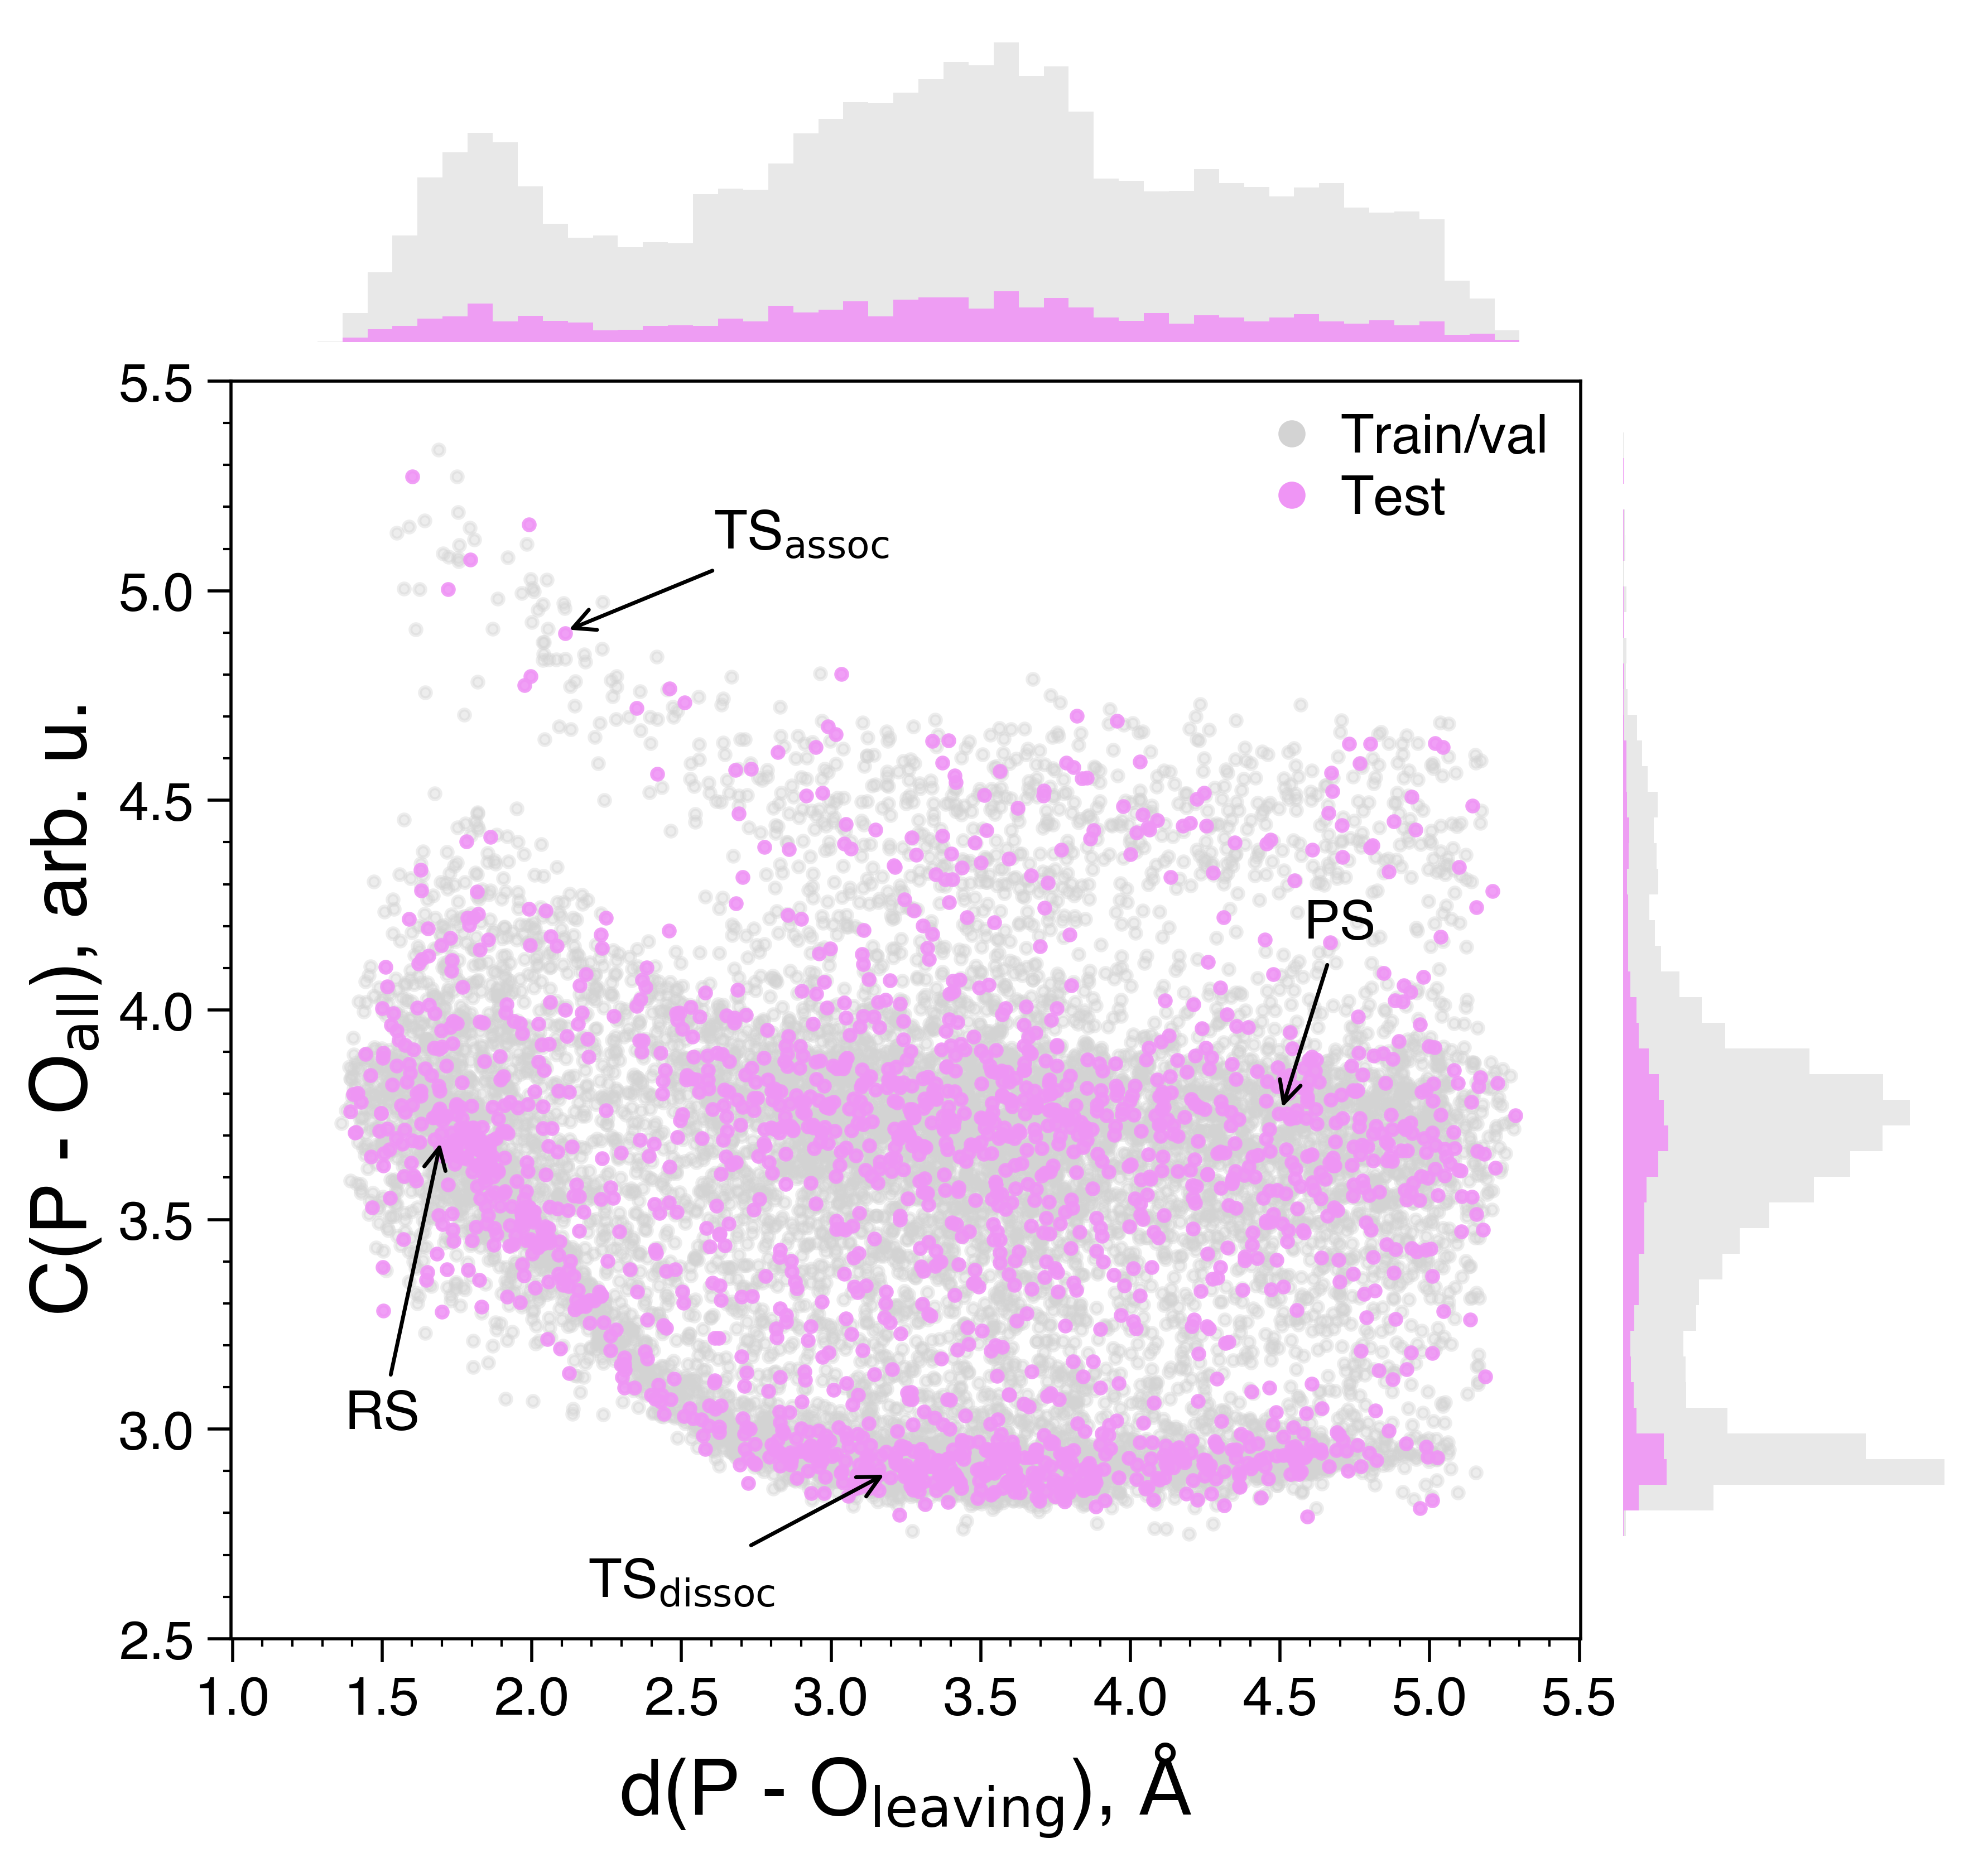
\includegraphics[width=0.9\textwidth]{Figures/4_Results/results_final_dataset_with_histograms.png}
    \caption{Left panel: final dataset composition projected on the two \acp{cv} space. RS stands for the reactant state, PS for the product state, and TS for the transition state. 50 bins were used to produce the histograms. Right panel: normalised densities of the two \acp{cv} for the training/validation and test sets.}
    \label{fig:final_dataset}
\end{figure}

The final dataset was obtained after three iterations of a learning loop, as described in Section~\ref{subsec:iterative-training-of-the-neural-network-potential}. During each iteration, the dataset was expanded by adding points from different regions of the \ac{fes}. This was achieved by imposing constraints on the \acp{cv}. For instance, in the first iteration, sampling primarily targeted the reactant and product basins, while in the second iteration, the focus shifted towards the transition state regions. The final iteration was dedicated to exploring the \ac{fes} at elevated temperatures (e.g., 320 and 340~K) in order to enhance the configurational diversity of the dataset. Sampling at higher temperatures generally improves the \ac{cv} space coverage, as it allows the system to visit higher-energy regions.

The final dataset comprises 12,000 data points for the training and validation sets, and 1,800 points for the test set, as illustrated in the left panel of Figure~\ref{fig:final_dataset}.

The reactant basin is well-defined, appearing as a narrow region in the \ac{cv} space. In contrast, the product basin is broader due to the diffusion of products within the simulation cell.

The sampling quality of the \ac{ts} regions varies. The dissociative pathway is substantially better represented than the associative one. This difference arises from the fact that the associative path lies higher in energy and is therefore more difficult to access. Nevertheless, it is still represented by a number of points, meaning the fitted potential should be capable of describing it to some extent.

A particularly important aspect of dataset construction was the implementation of density-aware sampling. This approach was adopted for several reasons. First and foremost, the algorithm was used to ensure that the dataset is balanced in terms of the \acp{cv} distribution, as shown in the right panel of Figure~\ref{fig:final_dataset}. Secondly, it was employed to guarantee sufficient configurational diversity, i.e., the inclusion of points from various physically meaningful regions of the \ac{fes}, thereby enhancing the potential's ability to generalise. This is crucial, as the neural network potential must be capable of predicting energies and forces for any configuration along the reaction coordinate. Lastly, density-aware sampling was used to ensure that the test set reflects the overall reaction space well, thereby providing a reliable basis for critically evaluating the accuracy and performance of the trained potential.



%%%%%%%%%%%%%%%%%%%%%%%%%%%%%%%%%%%%%%%%%%%%%%%%%%%%%%%%%%%%%%%%%%%%%%%%%%%%%%%%
\section{Accuracy and performance of the neural network potential}

\begin{figure}[t]
    \centering
    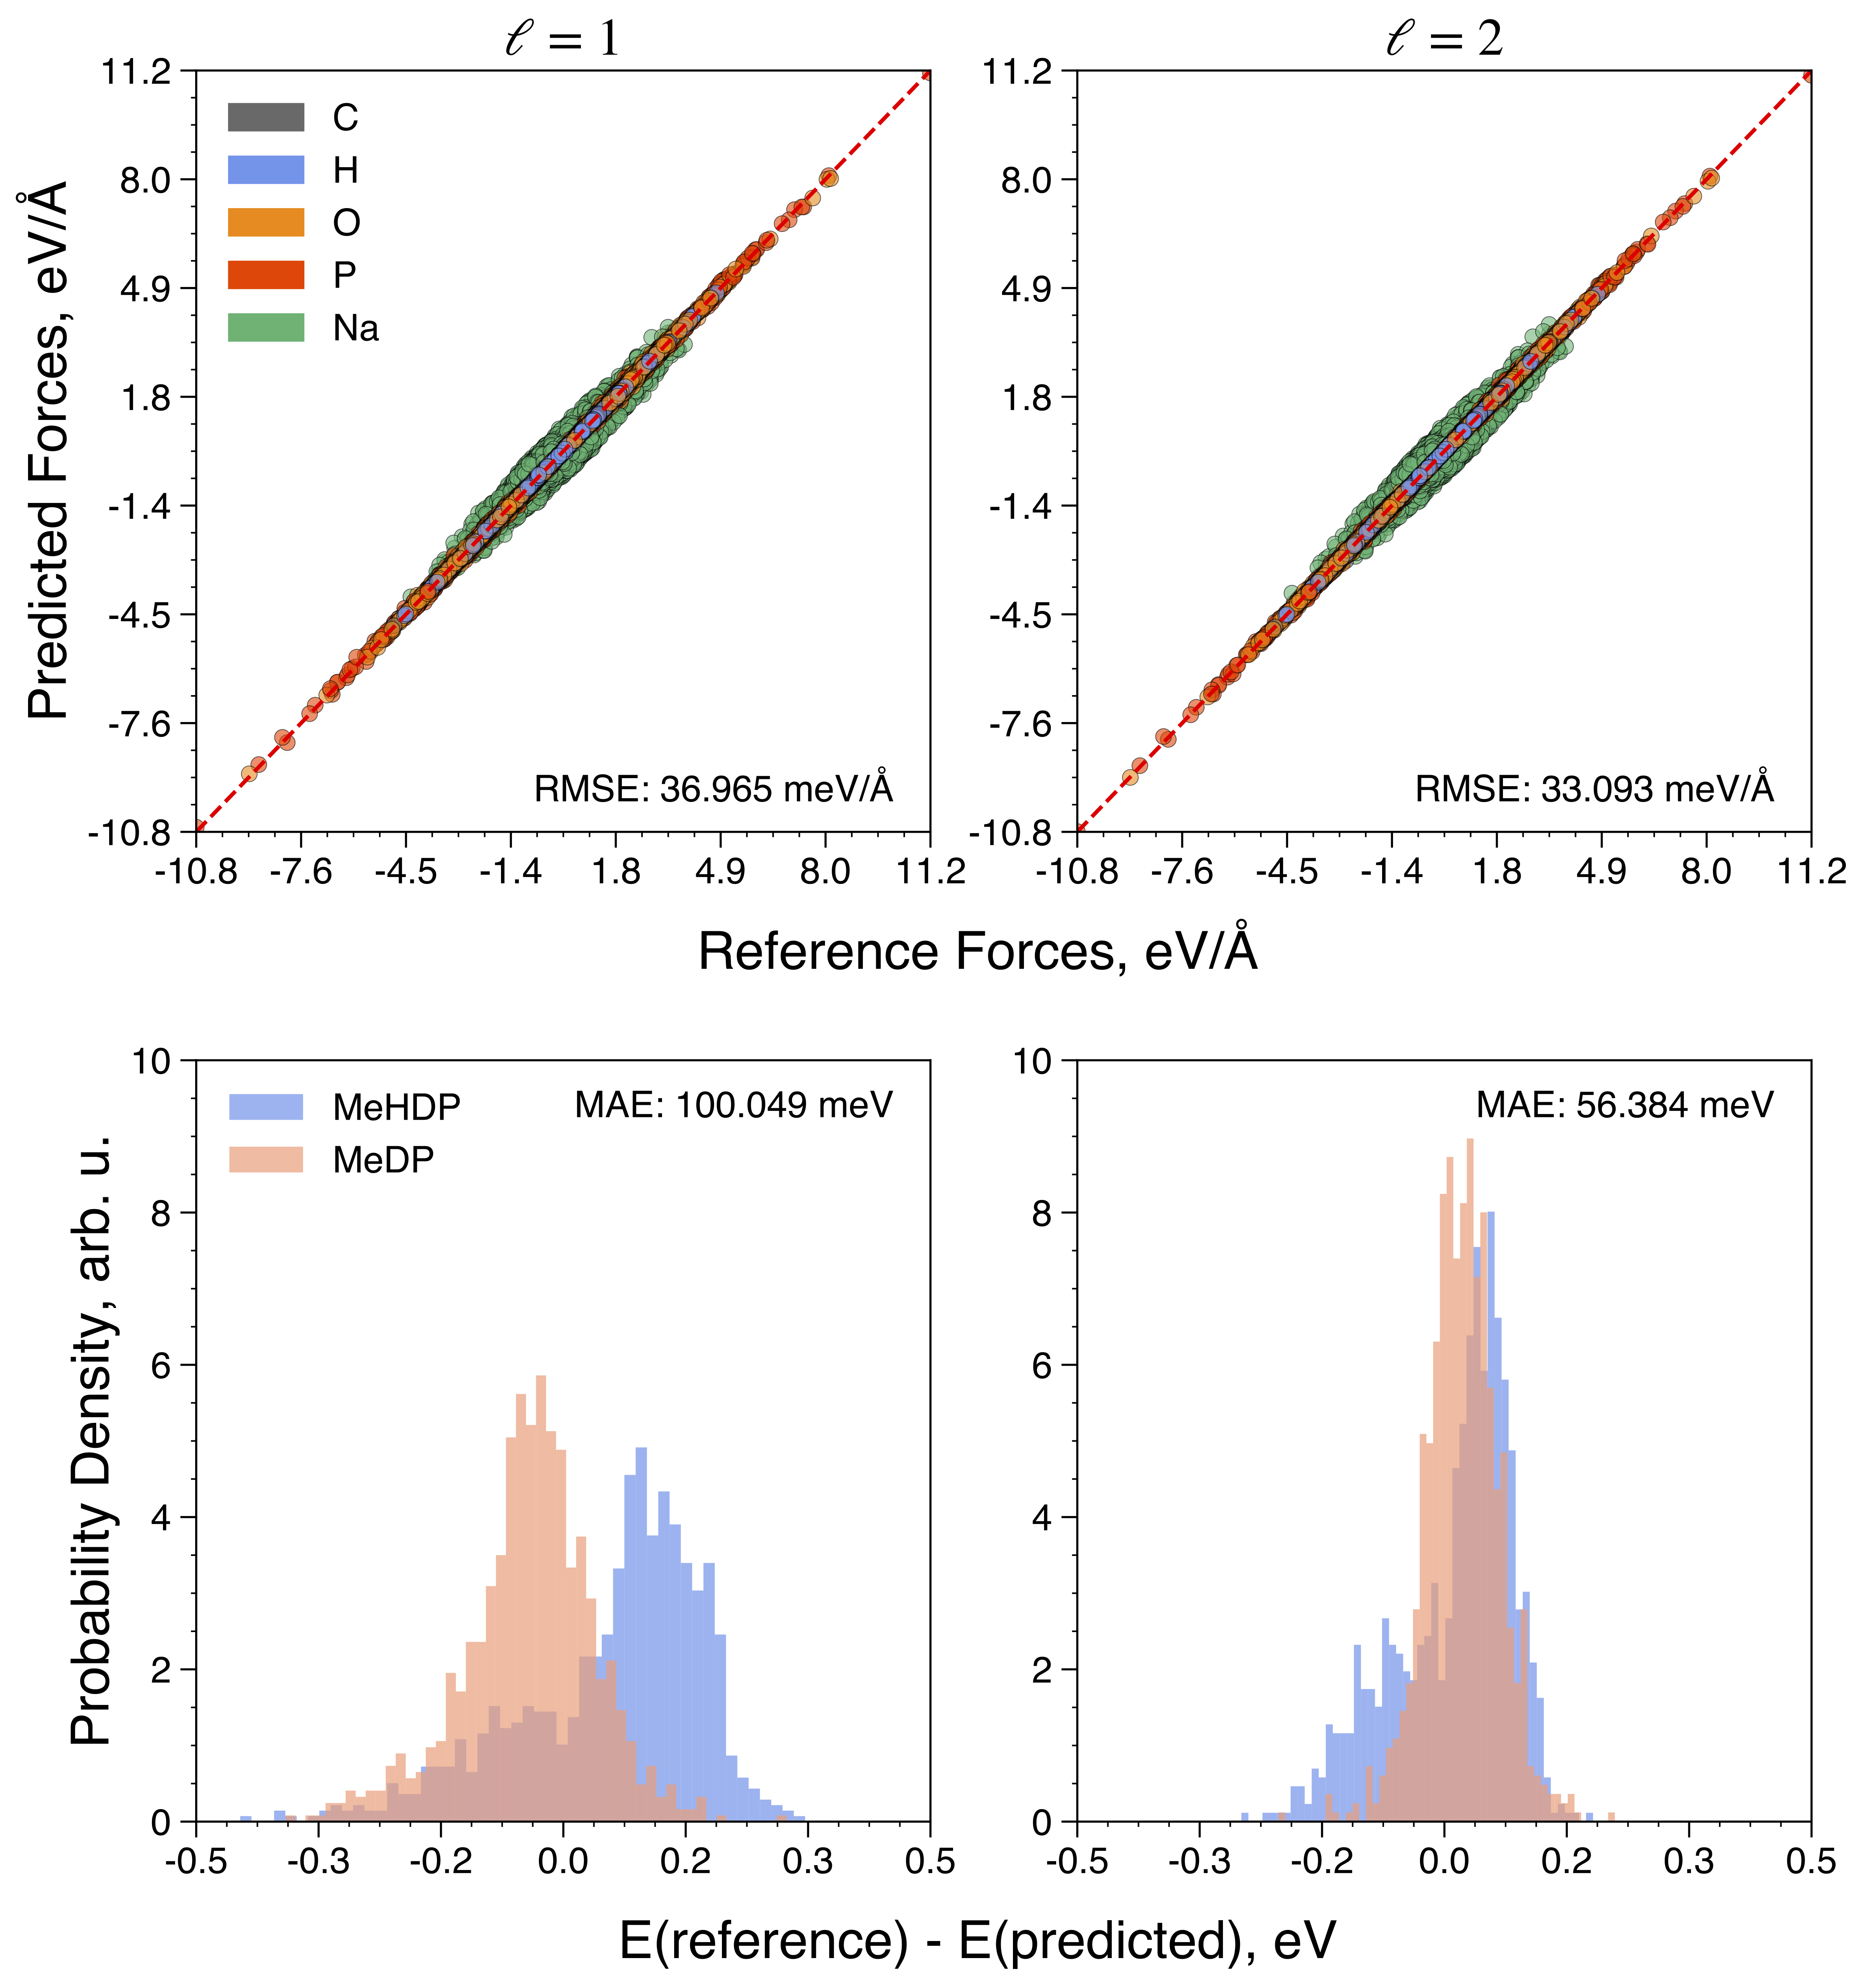
\includegraphics[width=0.8\textwidth]{Figures/4_Results/results_nnp_accuracy_l-1_l-2.png}
    \caption{Accuracy of the neural network potential trained on 12,000 data points. The left panel shows the errors in the forces and energy for the tensor rank $\ell=1$, and the right panel shows the errors for $\ell=2$. For the histograms, the number of bins was set to 50.}
    \label{fig:nnp_accuracy}
\end{figure}

At each iteration, the potential was fitted using a NequIP equivariant \ac{gnn} with a different tensor rank~$\ell$, namely $\ell=1$ and $\ell=2$ ($\ell=0$ would correspond to an invariant \ac{gnn}). The reason for using different tensor ranks was to investigate how the network complexity affects the accuracy of the potential. The tensor rank $\ell$ determines the number of parameters in the network, with higher values leading to more complex node representations.

The final potential was trained on 12,000 data points, and its accuracy is illustrated in Figure~\ref{fig:nnp_accuracy}. The left panel shows the errors in the forces and energy for tensor rank $\ell=1$, while the right panel shows the corresponding errors for $\ell=2$. The errors are calculated as the difference between the neural network potential and the reference \ac{dft} values.

According to current community standards~\citep{jacobsPracticalGuideMachine2025a}, the accuracy of a neural network potential is considered a `very good fit' when the \ac{rmse} in the forces lies within the range of 20-40~meV/\AA\ and the \ac{mae} in the energy is between 1-10~meV/atom. A `very accurate fit' is defined as the \ac{rmse} in the forces of approximately 10~meV/\AA\ and the \ac{mae} in the energy on the order of 1~meV/atom.

The \acp{nnp} obtained in this work fall somewhere in between these two categories. The \ac{rmse} in the forces is 37.069~meV/\AA\ for $\ell=1$ and 33.142~meV/\AA\ for $\ell=2$, while the \ac{mae} in the energy is below 0.3~meV/atom for $\ell=1$ and below 0.15~meV/atom for $\ell=2$.

As shown in Figure~\ref{fig:nnp_accuracy}, the errors in the forces lie along the diagonal, which represents a perfect fit. The only points that are slightly scattered correspond to sodium cations (Na\textsuperscript{+}) jiggling in solution, not being technically bound to anything. This makes it more challenging for the network to predict the forces on them.

Regarding the energy predictions, the potential with $\ell=1$ slightly overestimates them. This can be seen from the tail of the probability density on the left-hand side. The error appears to be systematic, meaning that when the \ac{nnp} encounters new points close to those in the training data, it would produce a consistent error that may cancel out when evaluating energy differences. In contrast, the potential with $\ell=2$ shows normally distributed energy errors, with no significant outliers. The histograms of the errors also demonstrate that the distributions are centred around zero, indicating that the potential does not systematically over- or under-estimate the energies and forces.

Overall, both potentials are very accurate, especially considering that they were trained on a fairly small dataset of 12,000 data points. This fact supports the idea that equivariant \acp{gnn} are indeed data-efficient. For instance, a related study~\citep{benayadPrebioticChemicalReactivity2024} investigated phosphoester bond formation between orthophosphate and methanol in bulk water. In that case, to achieve force errors on the order of 50~meV/\AA/atom, the authors had to train an invariant neural network, DeePMD~\citep{zengDeePMDkitV2Software2023}, on 220,000-400,000 data points.

It is important to note that the potentials are only as accurate as can be assessed by the test set, which contains 1,800 points spanning the entire \ac{fes} of the reaction. The test set was not used during training nor clashes with the training points, which confirms that the \ac{nnp} generalises well to unseen data.

\begin{figure}[t]
    \centering
    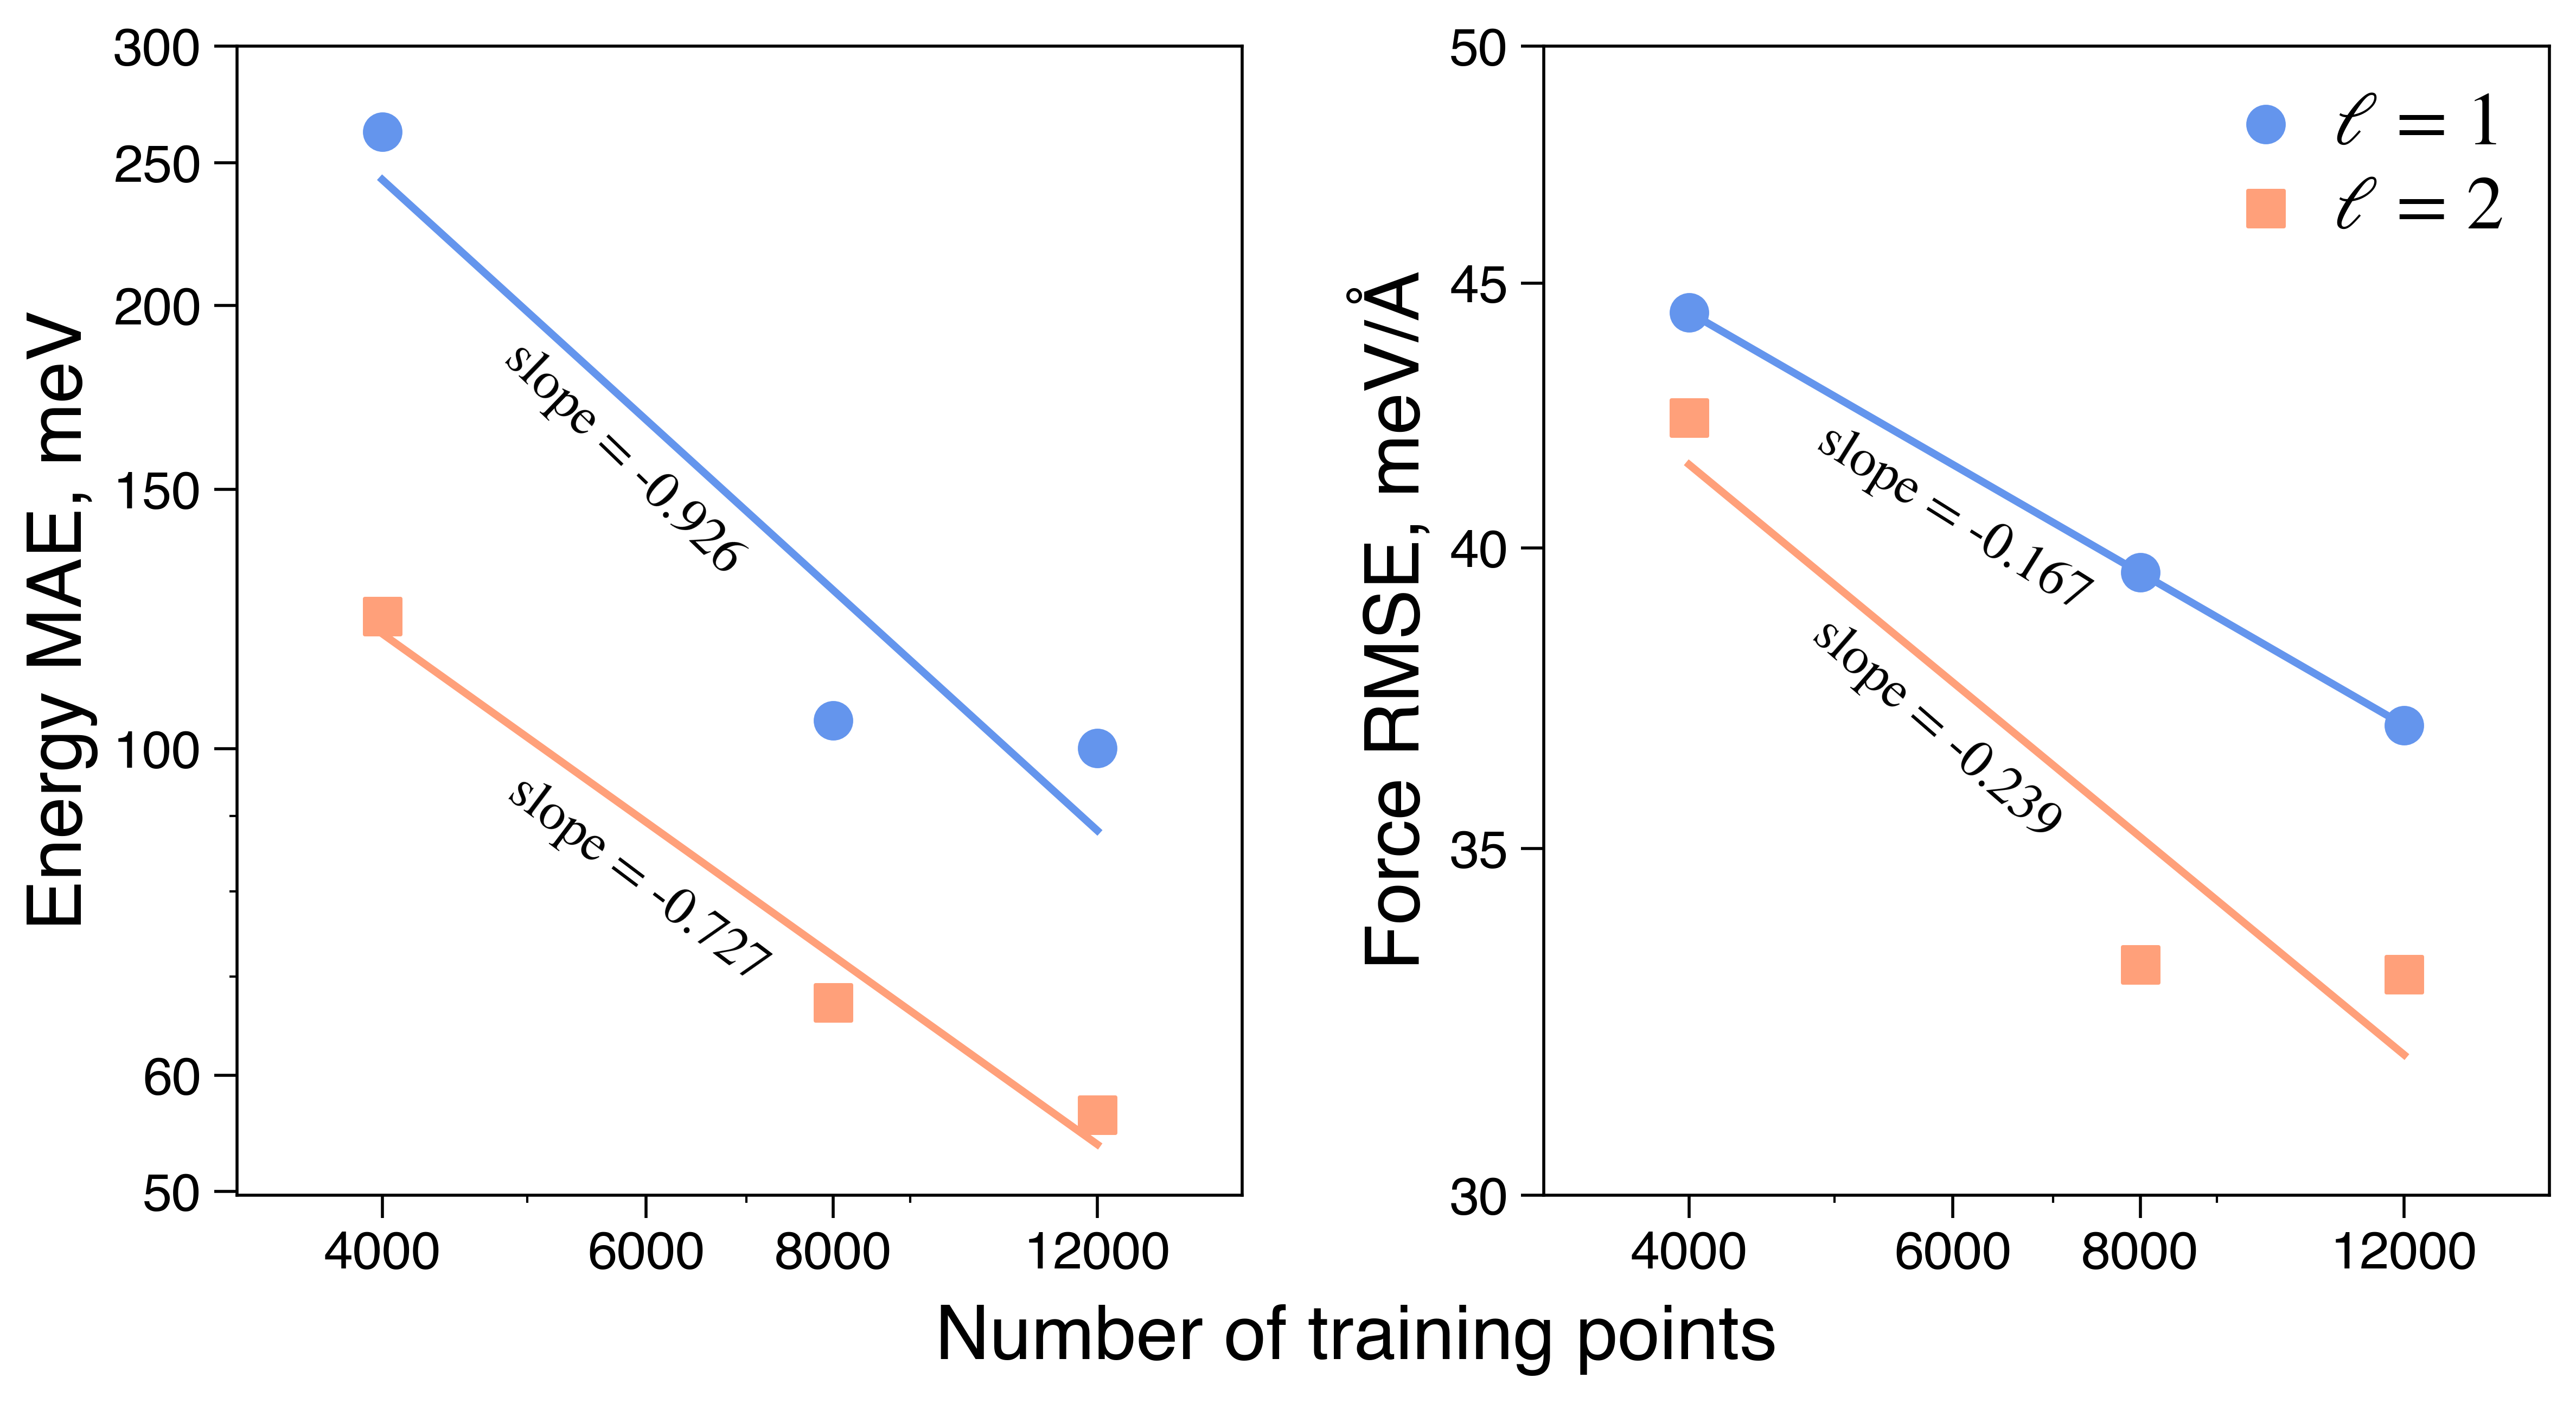
\includegraphics[width=0.8\textwidth]{Figures/4_Results/results_nnp_loglog_energy_force.png}
    \caption{Log-log plot of the errors in the energy and forces for the neural network potential with respect to the training dataset size. In all cases, the errors were calculated on the final test set of 1,800 data points.}
    \label{fig:nnp_log-log}
\end{figure}

The generalisability of the potentials can be further assessed by analysing how the errors in the energy and forces vary with the training dataset size. Figure~\ref{fig:nnp_log-log} shows a log-log plot of these errors for the \ac{nnp} at each iteration of the learning loop. The errors were evaluated \textit{a posteriori} on the final test set of 1,800 data points.

By examining the slopes, it becomes evident that the dataset size significantly influences how well the network learns the energies. The errors in the forces, however, are less sensitive to dataset size, which is reasonable given that the forces are not predicted directly by the network, but rather computed as the derivative of the energy with respect to atomic positions. Interestingly, the \acp{nnp} began producing sufficiently accurate results after the second training round, i.e., with 8,000 data points. This suggests that a dataset of 12,000 points is indeed sufficient to achieve a very good fit.

\begin{figure}[t]
    \centering
    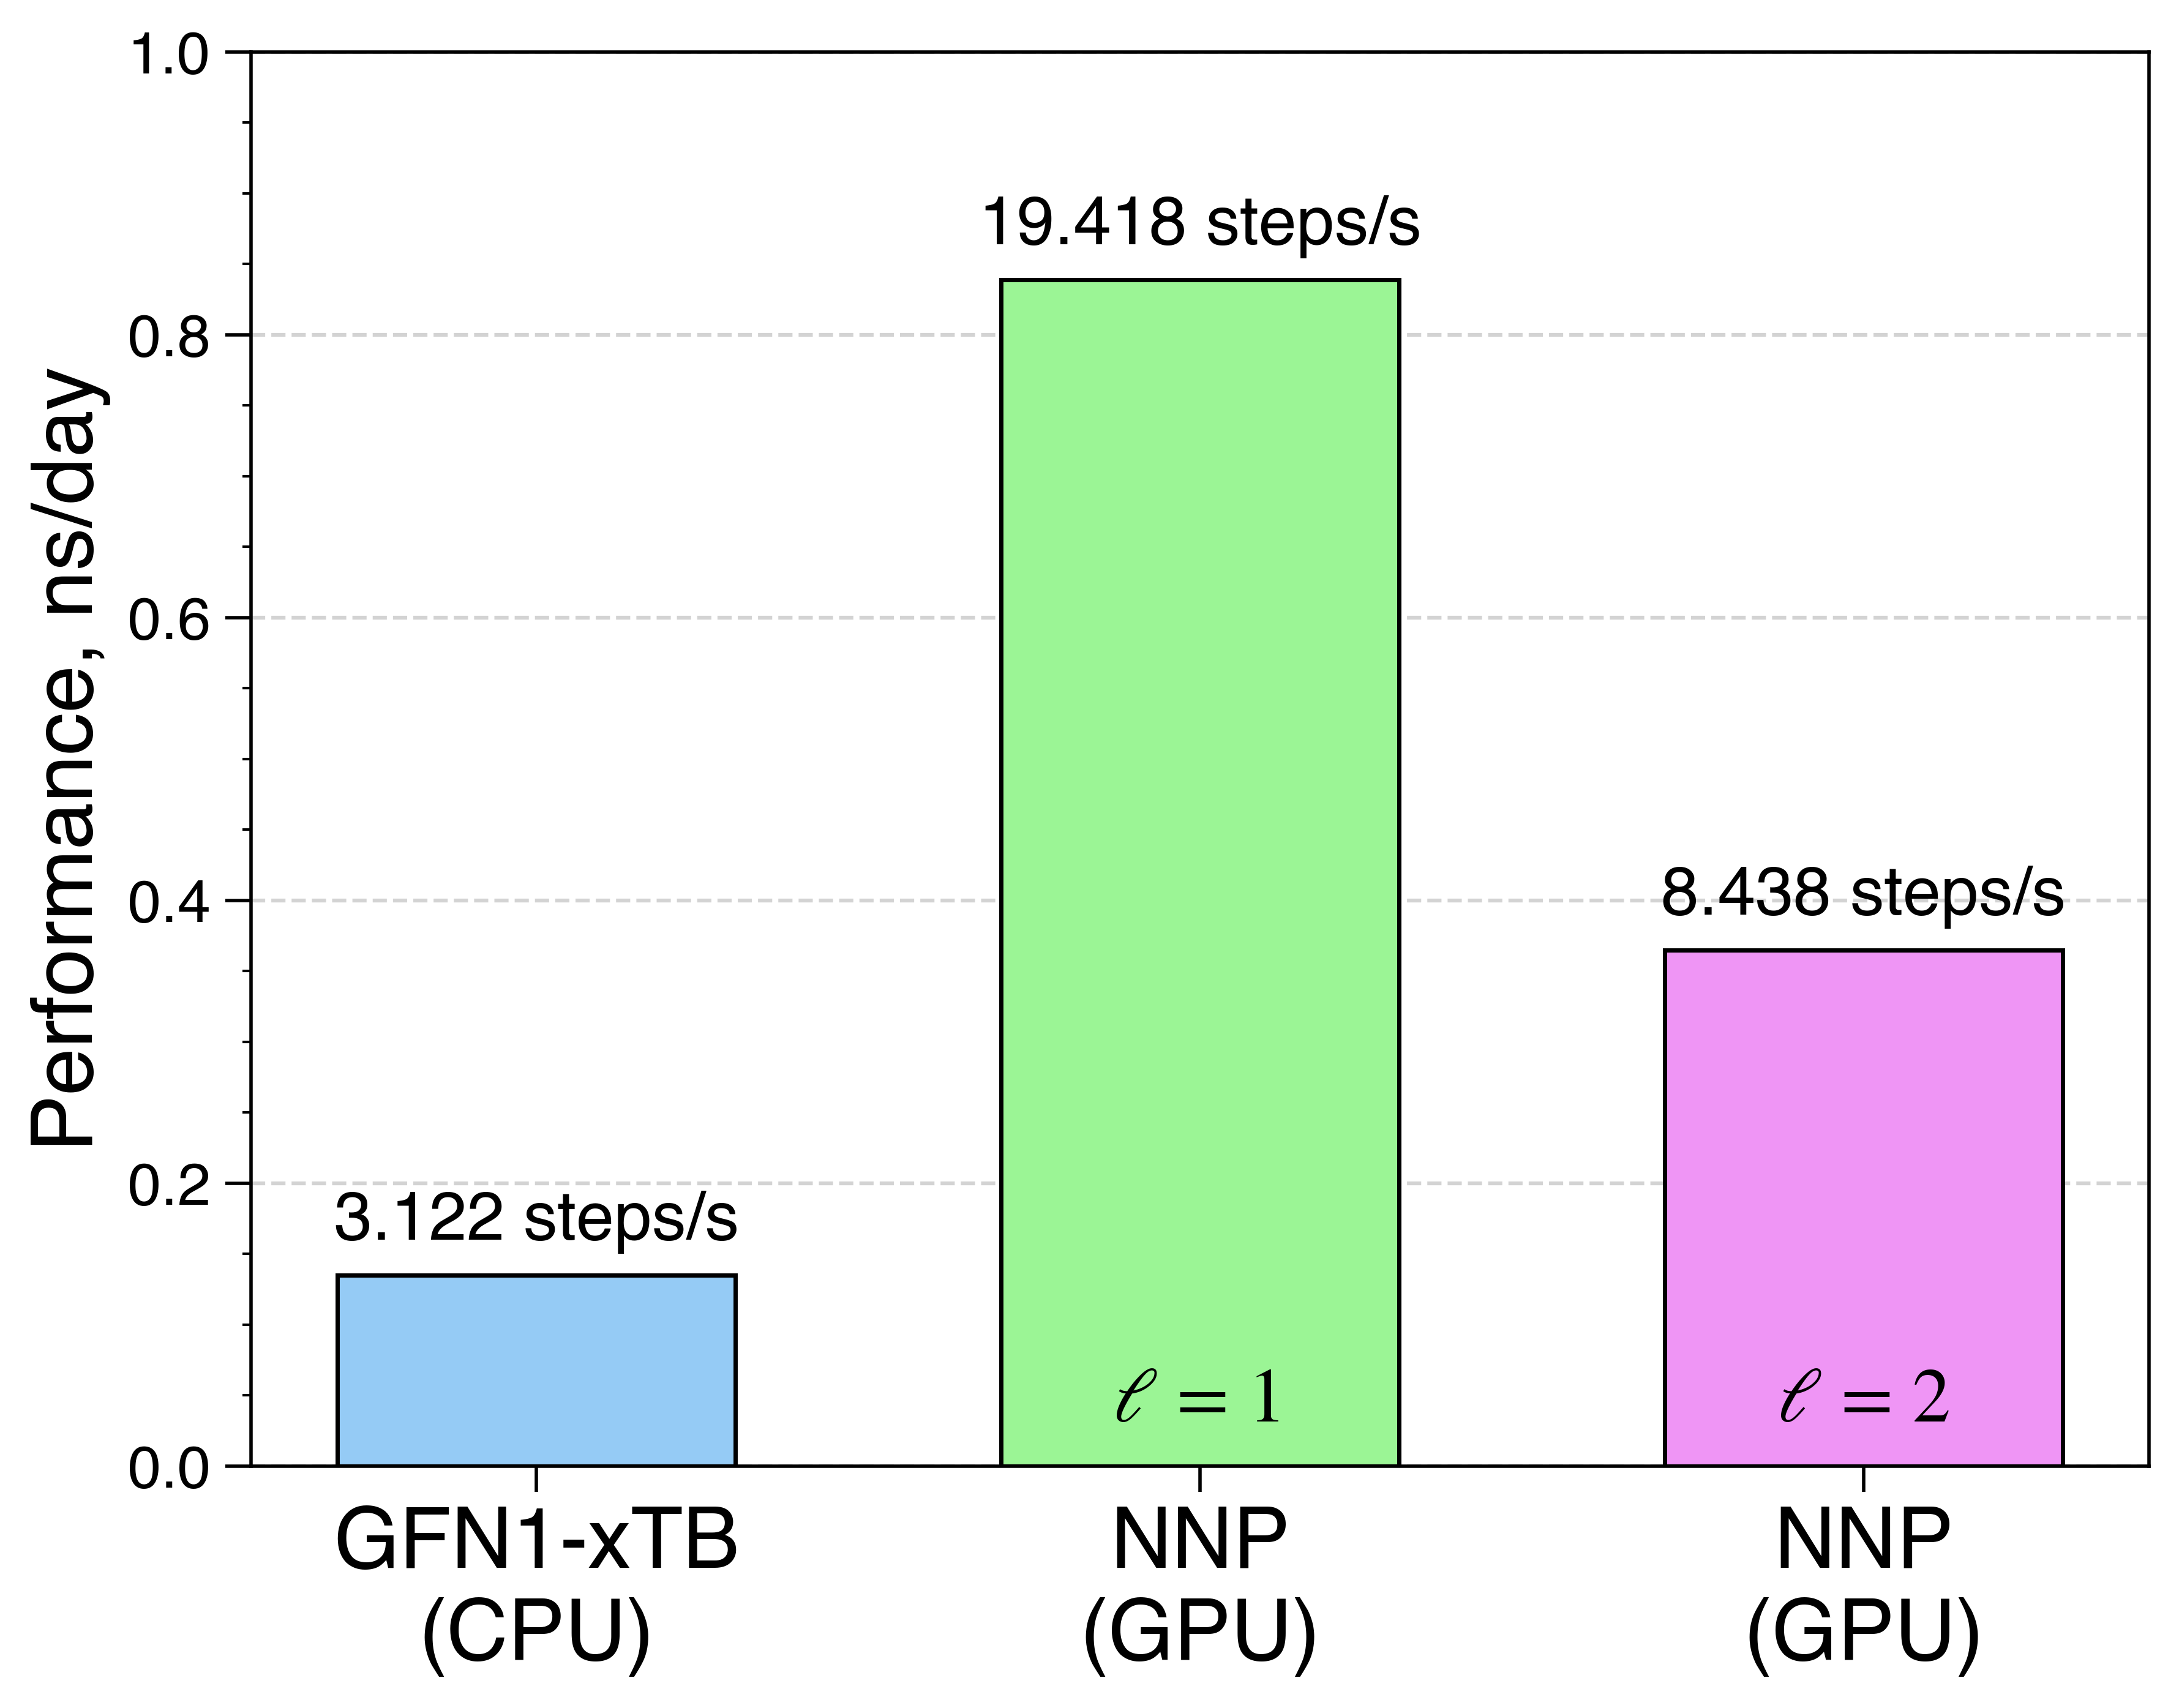
\includegraphics[width=0.6\textwidth]{Figures/4_Results/results_performance_comparison.png}
    \caption{Comparison of the performance between the \textit{ab initio} molecular dynamics runs driven by GFN1-xTB and neural network potentials fitted with different tensor ranks. CPU = 2 Intel Xeon Platinum 8468 CPUs (Sapphire Rapids), 48 cores each. GPU = 1 NVIDIA A100 80~GB GPU.}
    \label{fig:performance_comparison}
\end{figure}

The next question to address is which of the two \acp{nnp} should be used in subsequent calculations. To answer this, the performance of the potentials was compared in terms of computational time required to run \ac{aimd} simulations. The results are presented in Figure~\ref{fig:performance_comparison}. The \ac{aimd} simulations were performed on the \ac{medp} system.

It is clear that the \ac{nnp} with $\ell=1$ is significantly more efficient than both the $\ell=2$ \ac{nnp} and GFN1-xTB. It is important to highlight that the number of trainable parameters in the $\ell=1$ \ac{nnp} is 206,520, whereas for $\ell=2$ it is 452,280, making the latter nearly twice as slow in evaluating energies and gradients. Most likely, the performance of the \ac{pbe} functional would be considerably slower - so much so that its bar would not appear on the plot.

Taking both accuracy and performance into account, the \ac{nnp} with $\ell=1$ was selected for further calculations. It is sufficiently accurate to describe the reaction mechanism, and fast enough to allow for extended \ac{aimd} simulations. The \ac{nnp} with $\ell=2$ could be used in future work if an even more accurate potential is required.



%%%%%%%%%%%%%%%%%%%%%%%%%%%%%%%%%%%%%%%%%%%%%%%%%%%%%%%%%%%%%%%%%%%%%%%%%%%%%%%%
\section{Stability of the production runs}

\begin{figure}[b!]
    \centering
    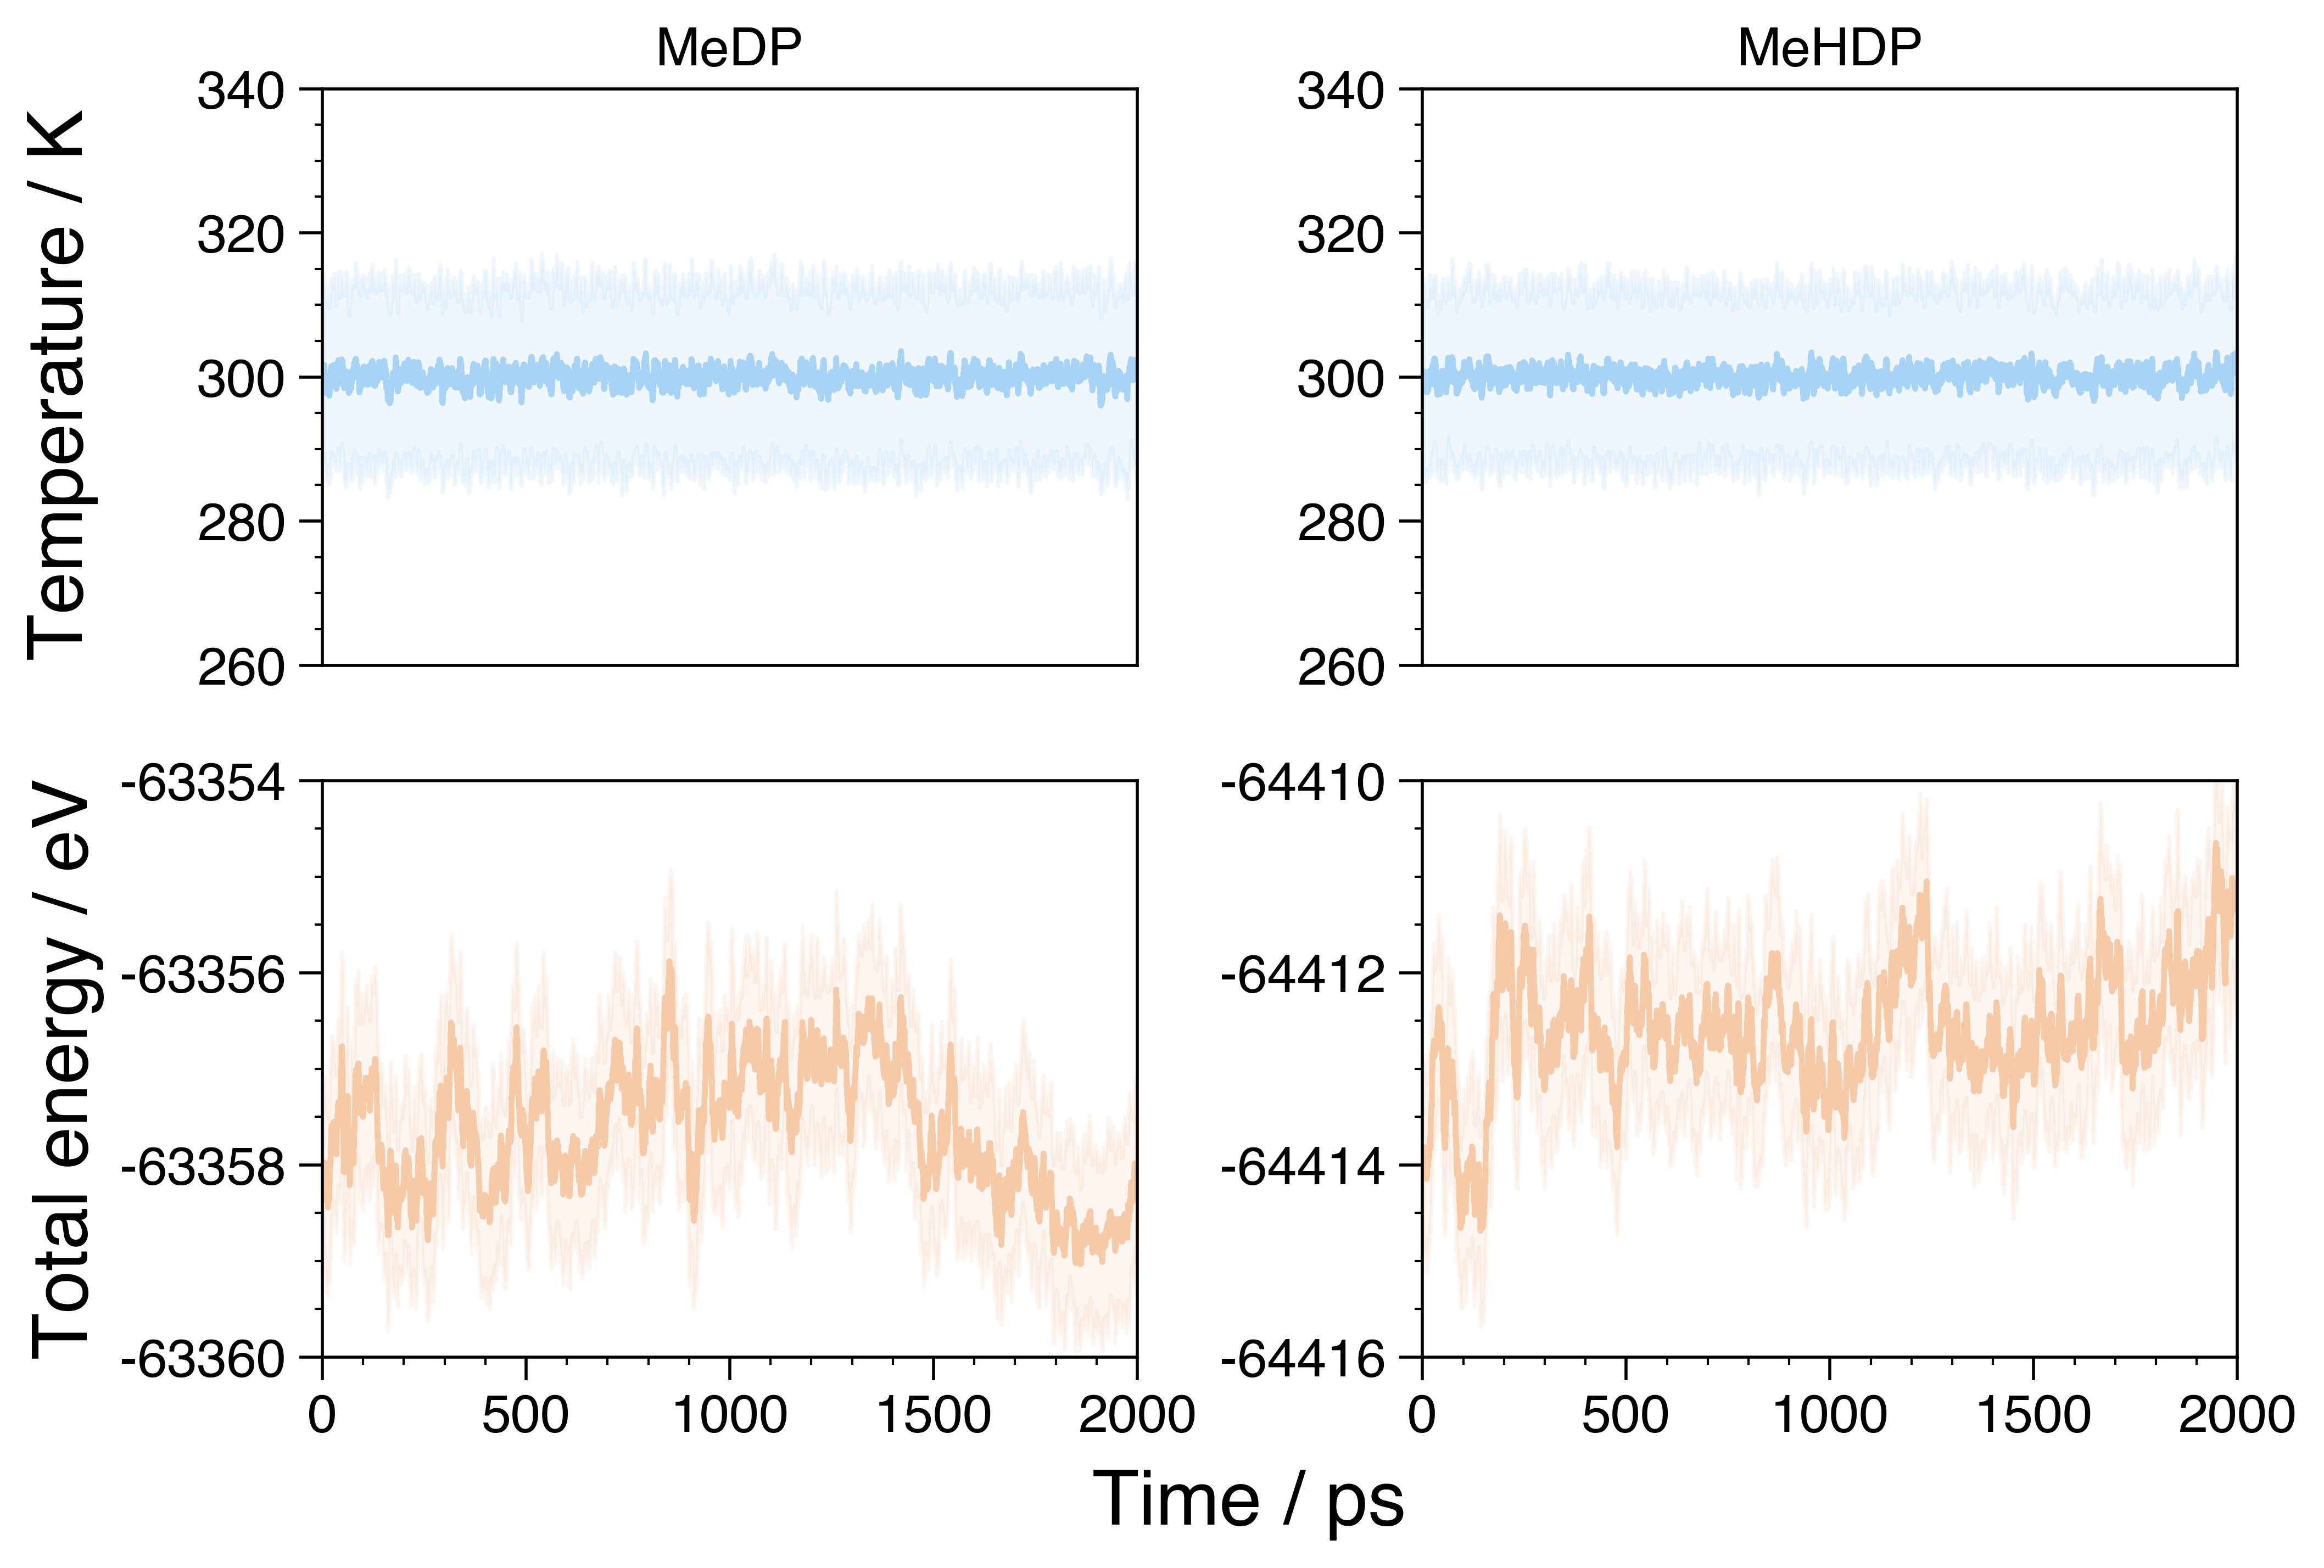
\includegraphics[width=0.8\textwidth]{Figures/4_Results/results_aimd_stability.png}
    \caption{Temperature and total energy fluctuations during the production runs at 300 K. The solid line represents the average, while the shaded area indicates the standard deviation. The average and the standard deviation were calculated using a sliding window of 1 ps.}
    \label{fig:temp_energy_fluctuations}
\end{figure}

Before discussing the reaction mechanism and the free energy profiles, it is important to assess the quality of the fitted \ac{nnp} in a real world scenario. To do so, we can briefly touch upon the stability of the production runs. The stability of the \ac{aimd} simulations was assessed by monitoring temperature and total energy fluctuations over time. The corresponding results are presented in Figure~\ref{fig:temp_energy_fluctuations}.

Temperature control was achieved using the Nos\'e--Hoover thermostat, while the total energy was calculated as the sum of potential and kinetic energies. The production runs were carried out at 300 K, and indeed, the average temperature remained close to this target, with a standard deviation of approximately 10 K. As expected for the \ac{nvt} ensemble, the total energy showed some fluctuations, yet remained within reasonable bounds in the simulations for both \ac{medp} and \ac{mehdp} systems.

It was of particular interest to evaluate the stability of the simulations driven by the \ac{nnp}. These simulations remained stable, exhibiting neither system explosions nor any other artefacts over the 4,000,000 time steps corresponding to 2 ns. This indicates the absence of extreme force values that could have caused numerical instabilities. In a recent study~\citep{fuForcesAreNot2023}, the authors compared the stability of \ac{aimd} simulations driven by equivariant and invariant \acp{nnp}, and found that NequIP was among the most stable potentials tested across various systems. The robustness of the fitted by NequIP \ac{nnp} employed in this work is consistent with those findings.



%%%%%%%%%%%%%%%%%%%%%%%%%%%%%%%%%%%%%%%%%%%%%%%%%%%%%%%%%%%%%%%%%%%%%%%%%%%%%%%%
\section{Radial distribution function of water}

\begin{figure}[b!]
    \centering
    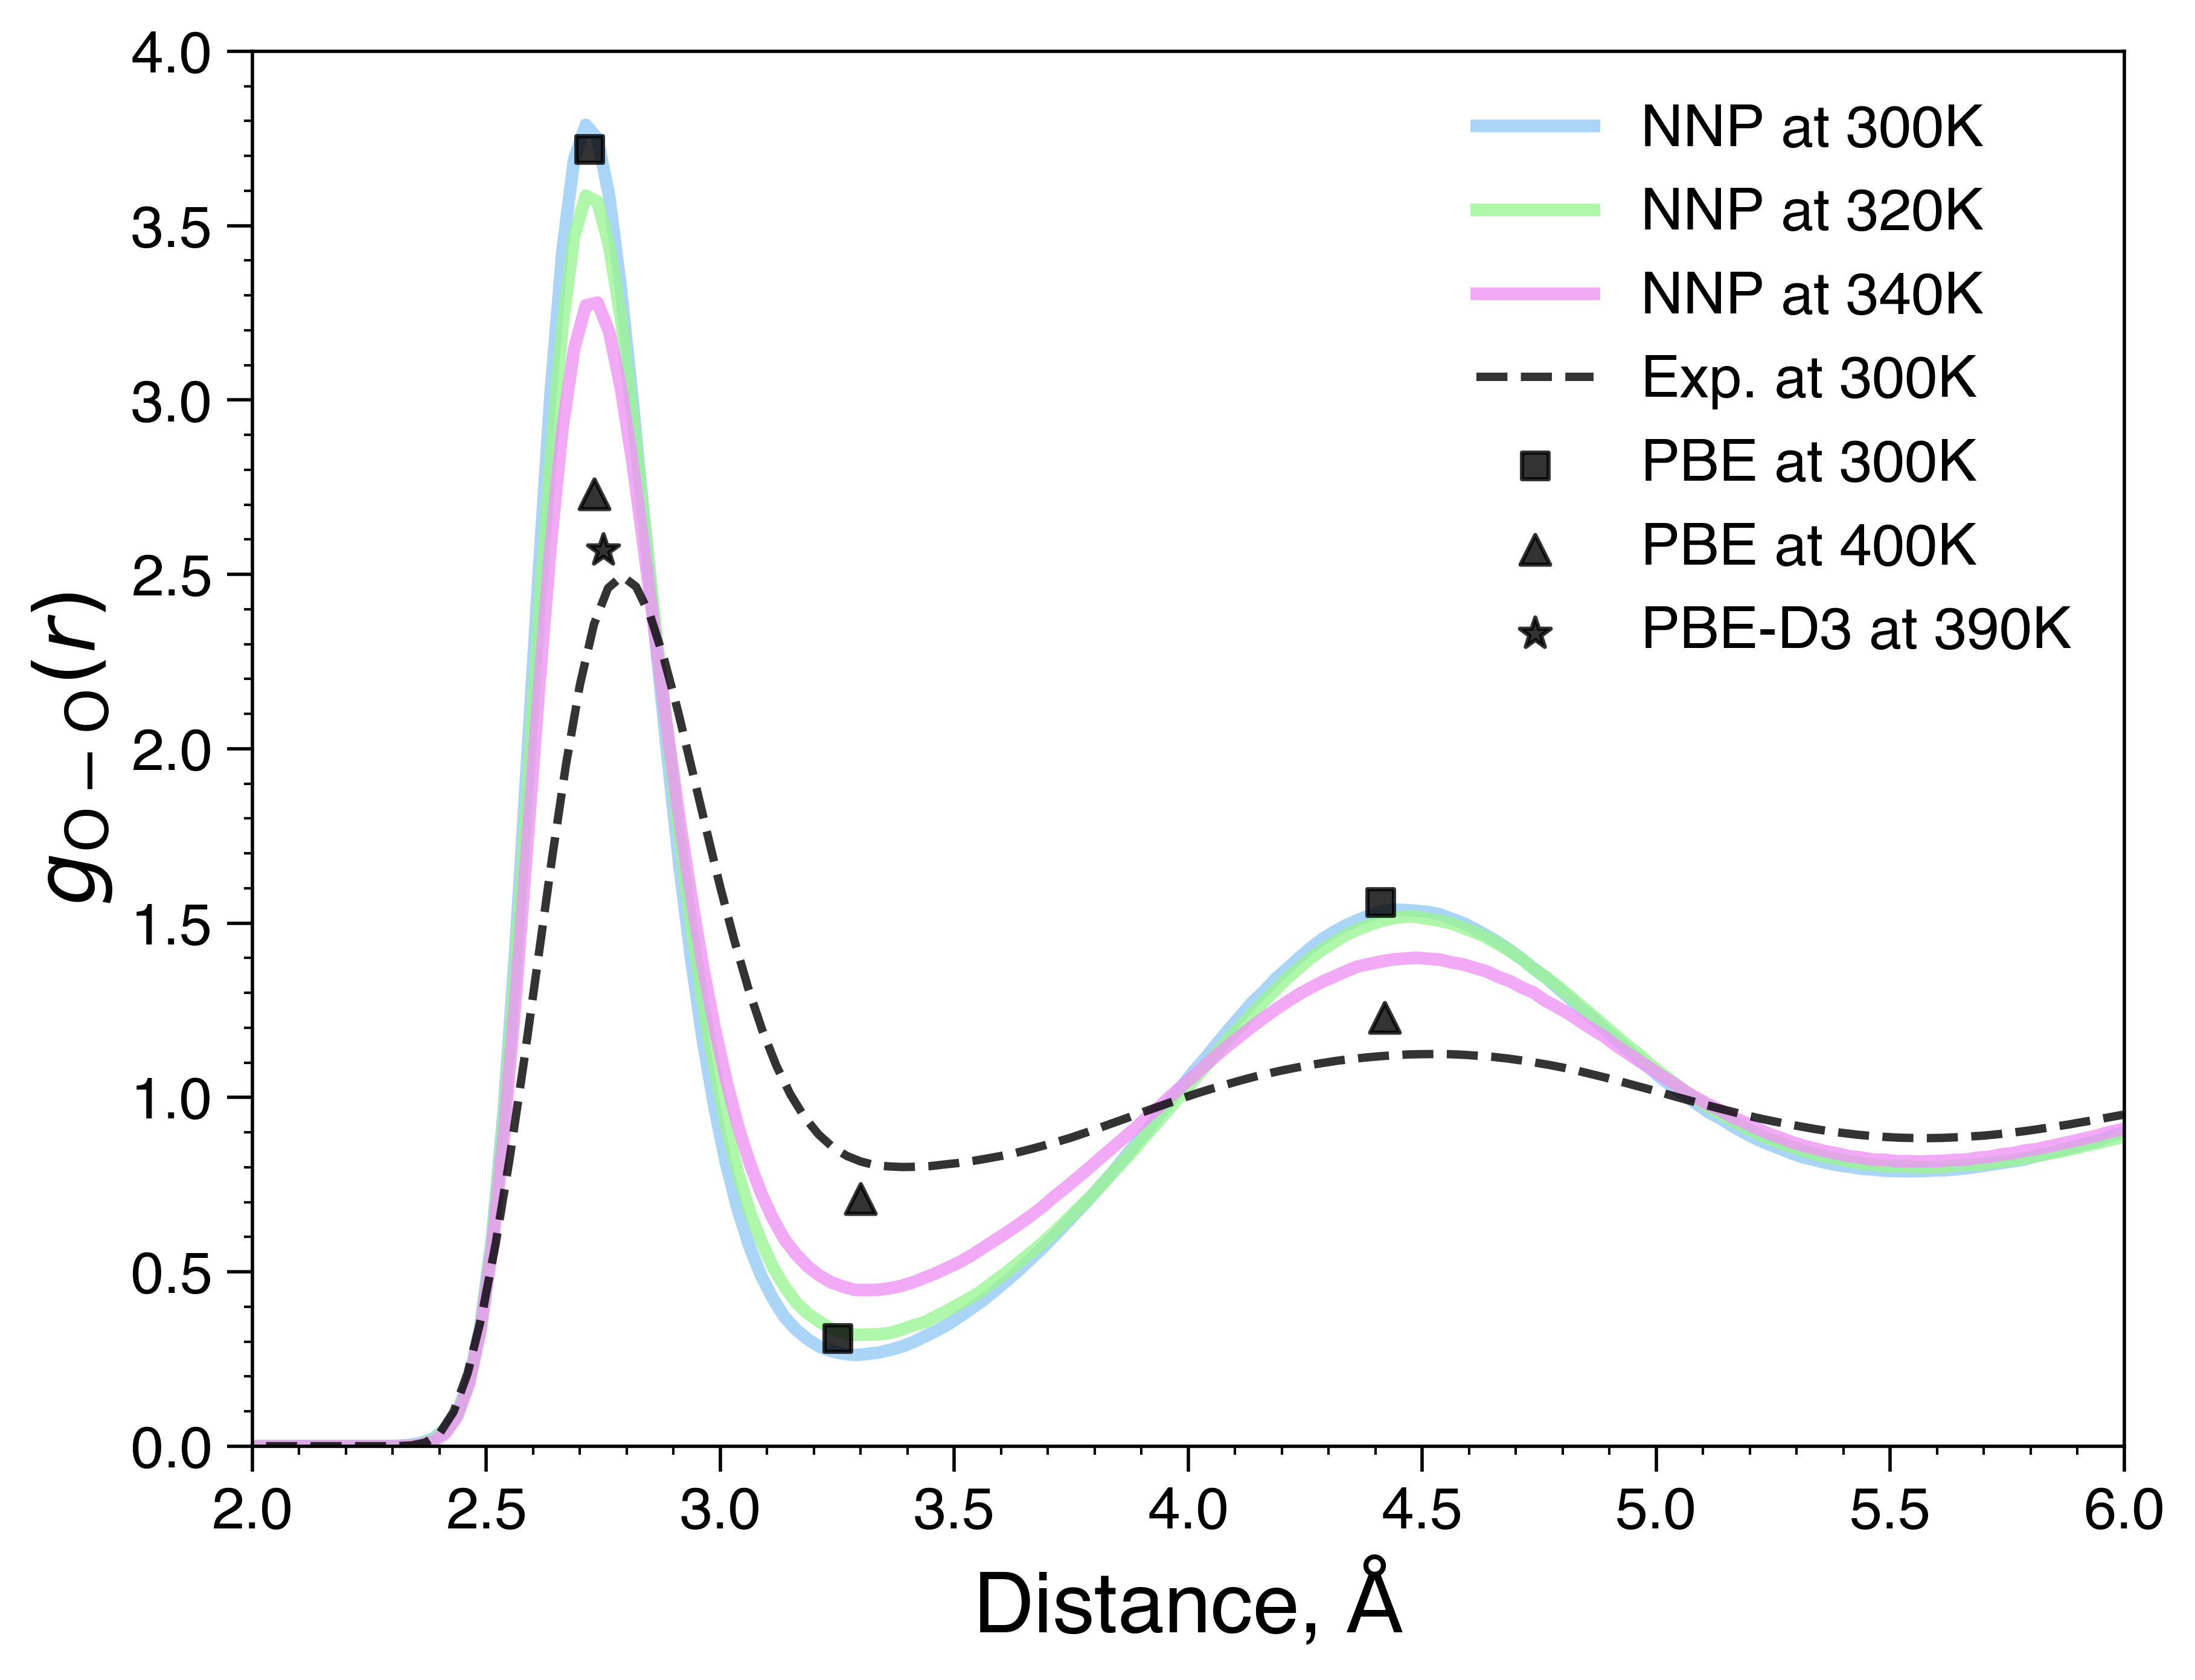
\includegraphics[width=0.6\textwidth]{Figures/4_Results/results_water_rdf.png}
    \caption{Oxygen-oxygen \ac{rdf} of water calculated from a production run at 300 K. Experimental data was taken from~\citep{soperRadialDistributionFunctions2013}. The PBE and PBE-D3 data were taken from \citep{phamStructureDynamicsAqueous2016} and \citep{zhouQuantifyingStructureWater2022}, respectively.}
    \label{fig:water_rdf}
\end{figure}

The quality of the \ac{nnp} can be further assessed by comparing the \ac{rdf} of water calculated from the production runs with experimental data and previously reported computational findings. The oxygen-oxygen RDF obtained from the \ac{medp} production run is shown in Figure~\ref{fig:water_rdf}.

It is evident that the \ac{nnp} is in qualitative agreement with the experimental data. However, it overestimates the heights of the first two peaks and underestimates the depth of the first minimum. For the \ac{nnp}, the first maximum occurs at 2.7188~\AA\ with a height of 3.8189, while the first minimum is located at 3.2813~\AA\ with a value of 0.2515. The second maximum appears at 4.4938~\AA\ with a height of 1.5725. There is also a slight shift to the left in the position of the peaks in comparison to the experimental data.

One could argue that the accuracy of the fitted \ac{nnp} is inherently limited by the quality of the training data. In this study, the dataset was labelled at the PBE-D3(BJ)/TZV2P level of theory. Accordingly, the resulting oxygen-oxygen water \ac{rdf} is consistent with the \ac{aimd} study where the \ac{rdf} was calculated using the \ac{pbe} functional~\citep{phamStructureDynamicsAqueous2016} as can be found in Figure~\ref{fig:water_rdf}.

It has previously been shown that, in order to obtain a more accurate representation of bulk water structure, the system temperature should be increased. For instance, \citep{zhouQuantifyingStructureWater2022} reported that the PBE functional with the Grimme's D3 dispersion correction yields a more accurate \ac{rdf} at 390 K. A similar trend was observed for the \ac{pbe} functional~\citep{phamStructureDynamicsAqueous2016}, with better agreement with experimental data achieved at 400 K.

In this work, the production runs were conducted at 300 K. Consequently, the resulting structure and dynamics of water will be less accurately captured than at elevated temperatures. Nevertheless, it remains in good agreement with what would be expected from the \ac{pbe} functional.



%%%%%%%%%%%%%%%%%%%%%%%%%%%%%%%%%%%%%%%%%%%%%%%%%%%%%%%%%%%%%%%%%%%%%%%%%%%%%%%%
\section{Convergence of the free energy profiles}



\begin{figure}[ht]
    \centering
    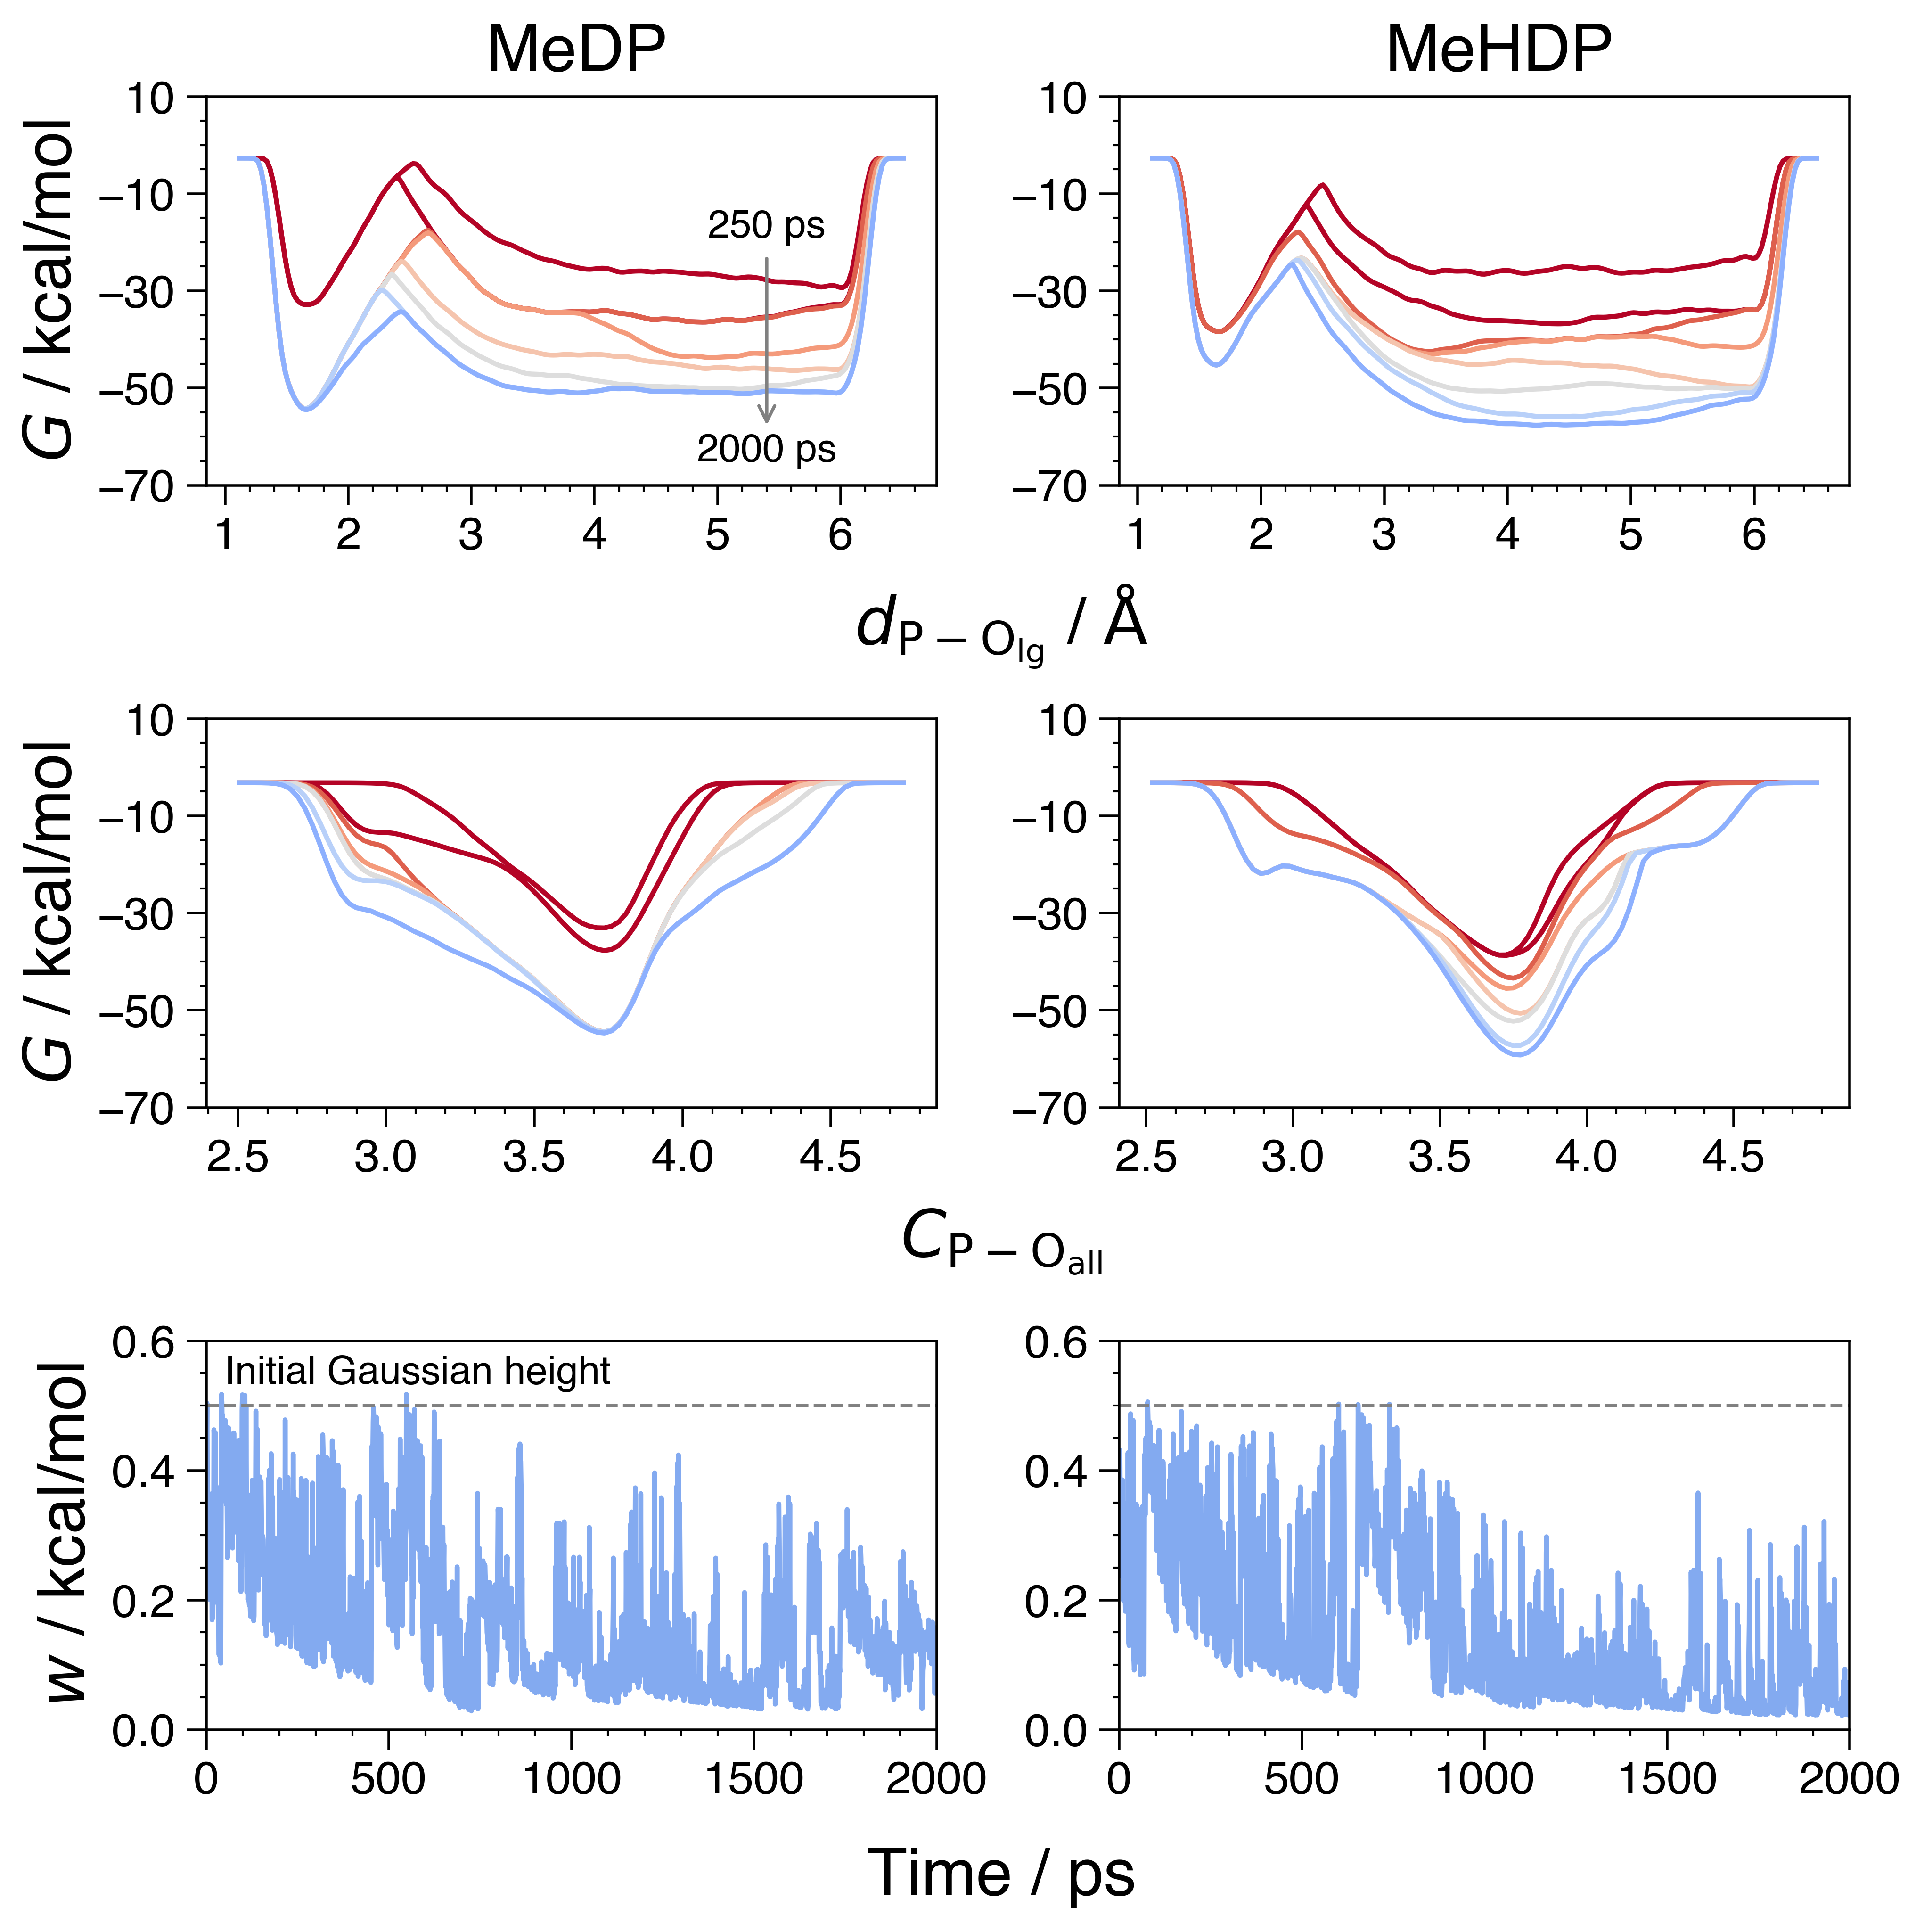
\includegraphics[width=0.9\textwidth]{Figures/4_Results/results_300K_fes_convergence.png}
    \caption{FES convergence at 300K}
    \label{fig:300k_fes_convergence}
\end{figure}



%%%%%%%%%%%%%%%%%%%%%%%%%%%%%%%%%%%%%%%%%%%%%%%%%%%%%%%%%%%%%%%%%%%%%%%%%%%%%%%%
\clearpage
\section{Evolution of the collective variables over time}

\begin{figure}[ht]
    \centering
    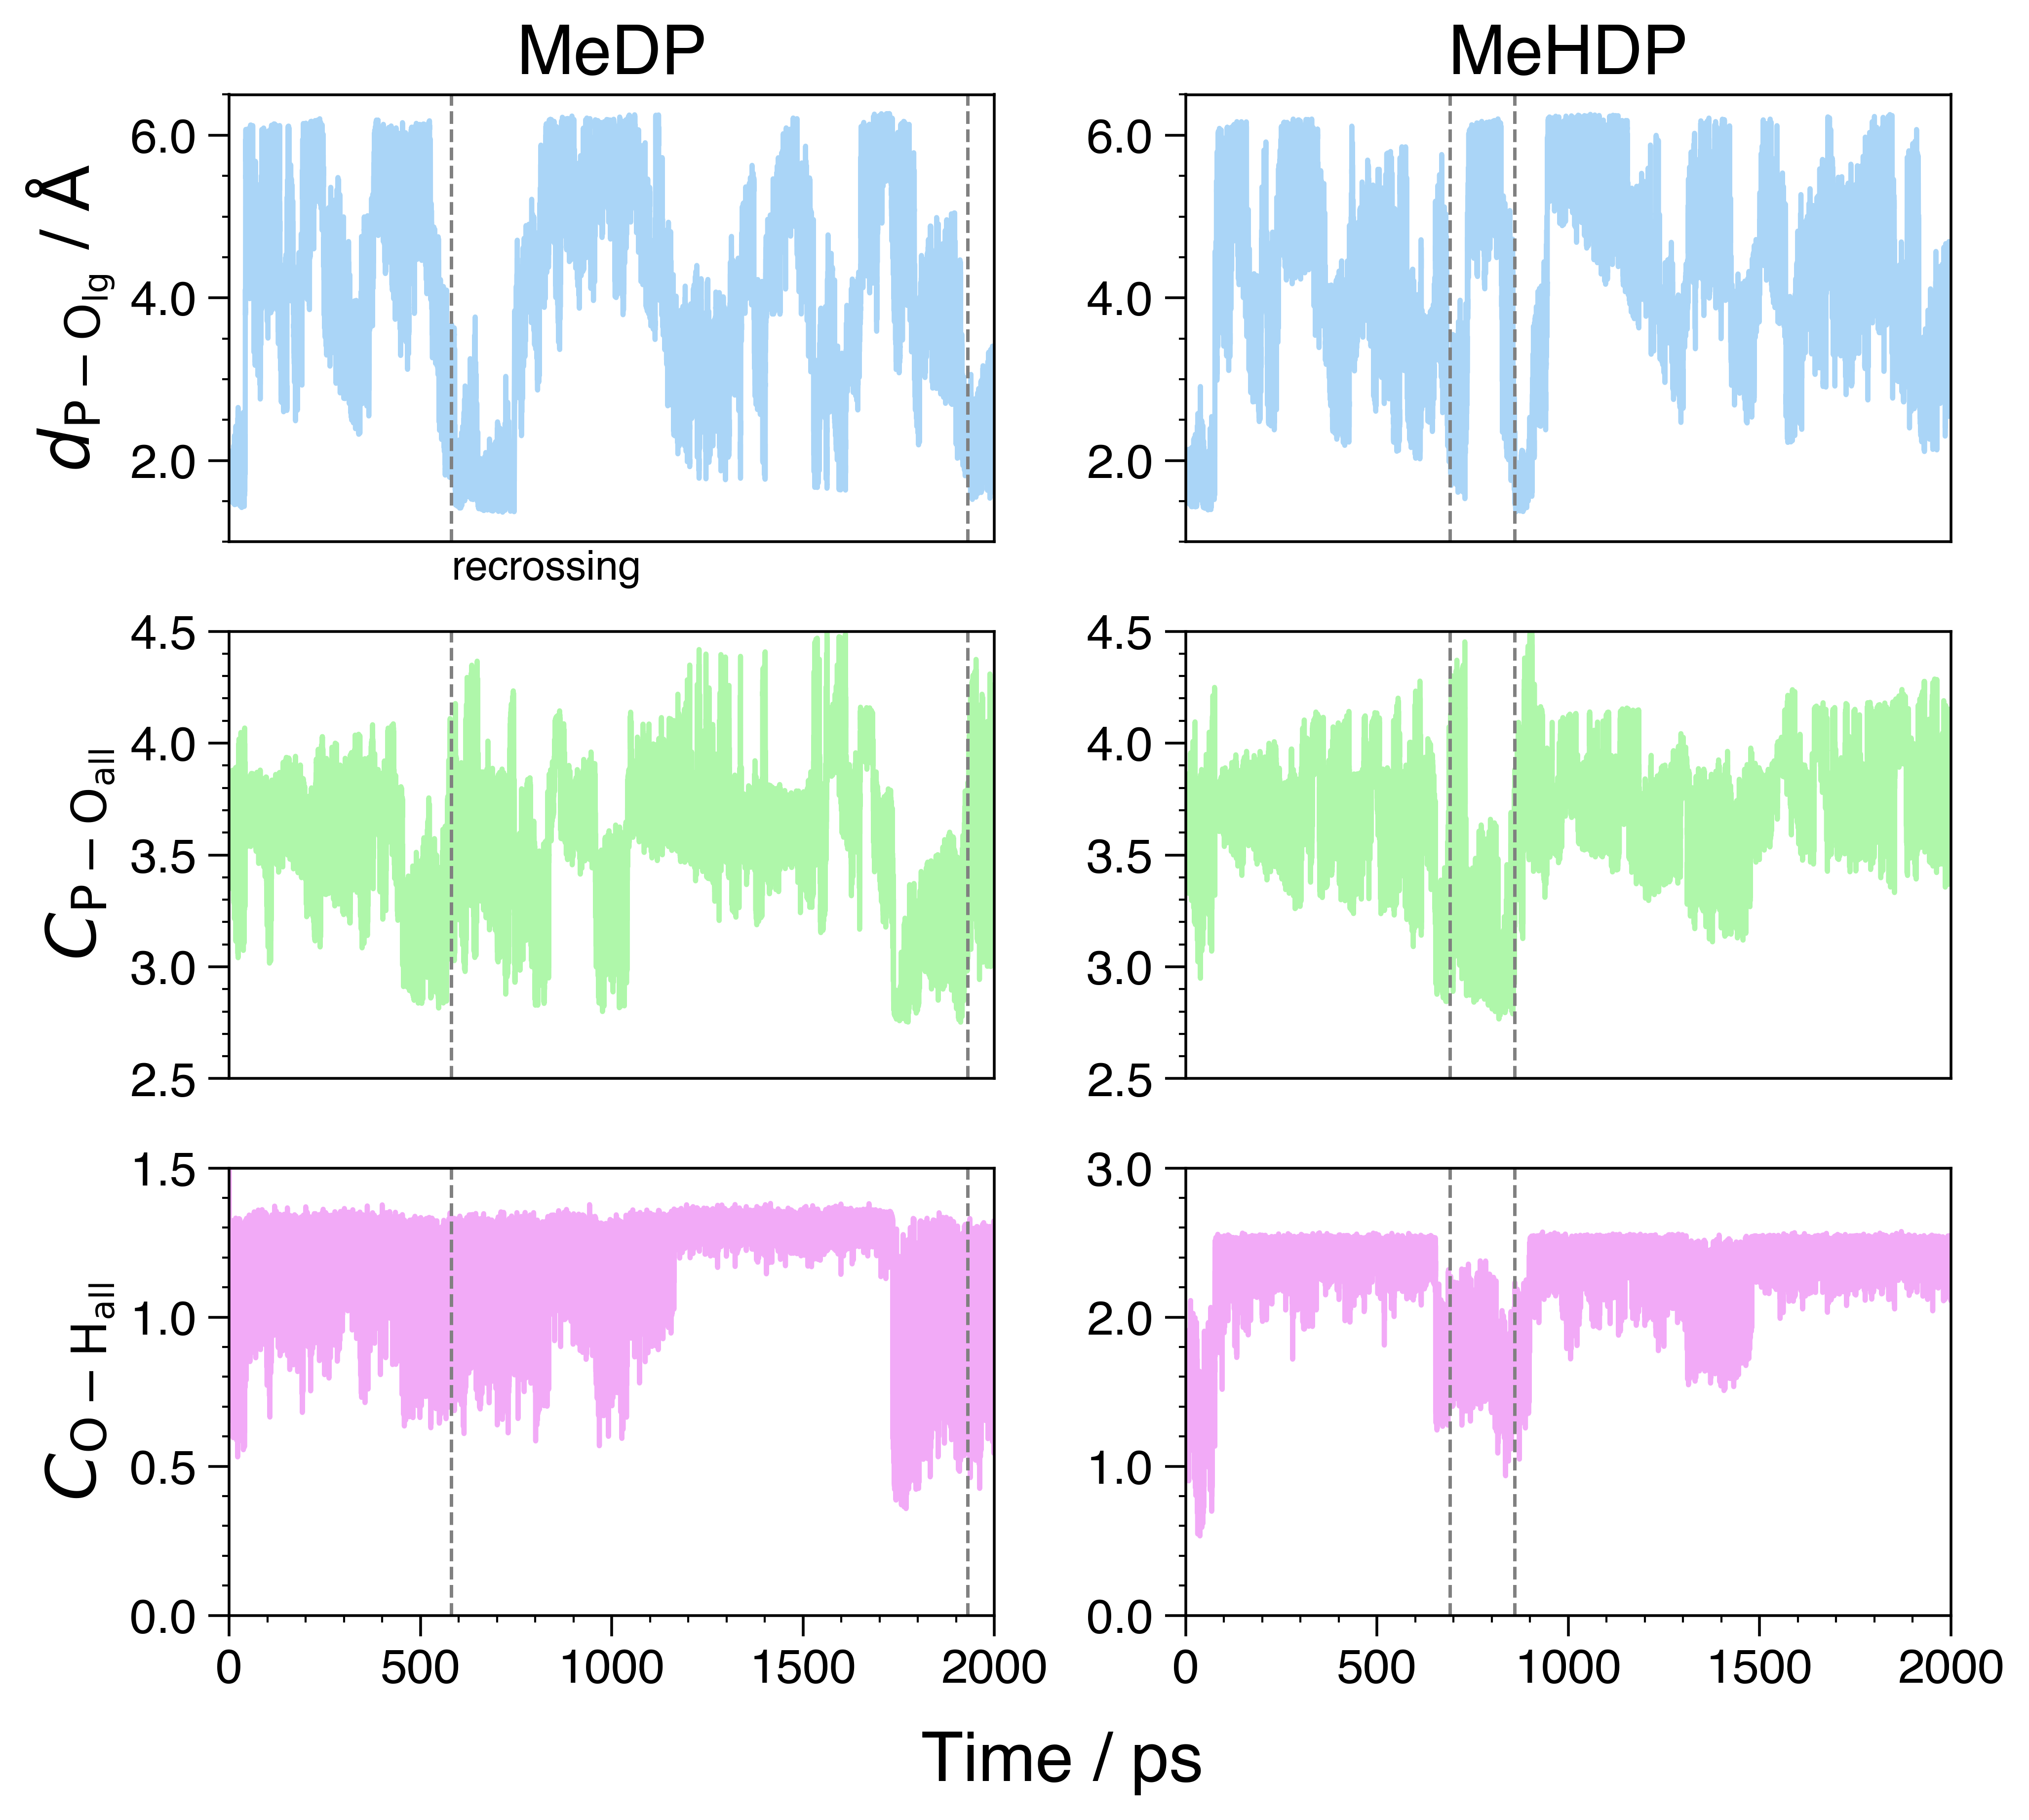
\includegraphics[width=0.9\textwidth]{Figures/4_Results/results_300K_cv_evolution.png}
    \caption{CV evolution at 300K}
    \label{fig:300k_cv_evolution}
\end{figure}



%%%%%%%%%%%%%%%%%%%%%%%%%%%%%%%%%%%%%%%%%%%%%%%%%%%%%%%%%%%%%%%%%%%%%%%%%%%%%%%%
\clearpage
\section{Reaction mechanism for methyl diphosphate trianion}

% MeDP
% RS -54.132690421
% PS -50.382700415

% TSassoc -20.983371369 29
% CN d
% 4.03 2.03

% TSdissoc -25.917009928 100
% CN d
% 2.92 3.32


\subsection{Minimum free energy path}

\begin{figure}[ht]
    \centering
    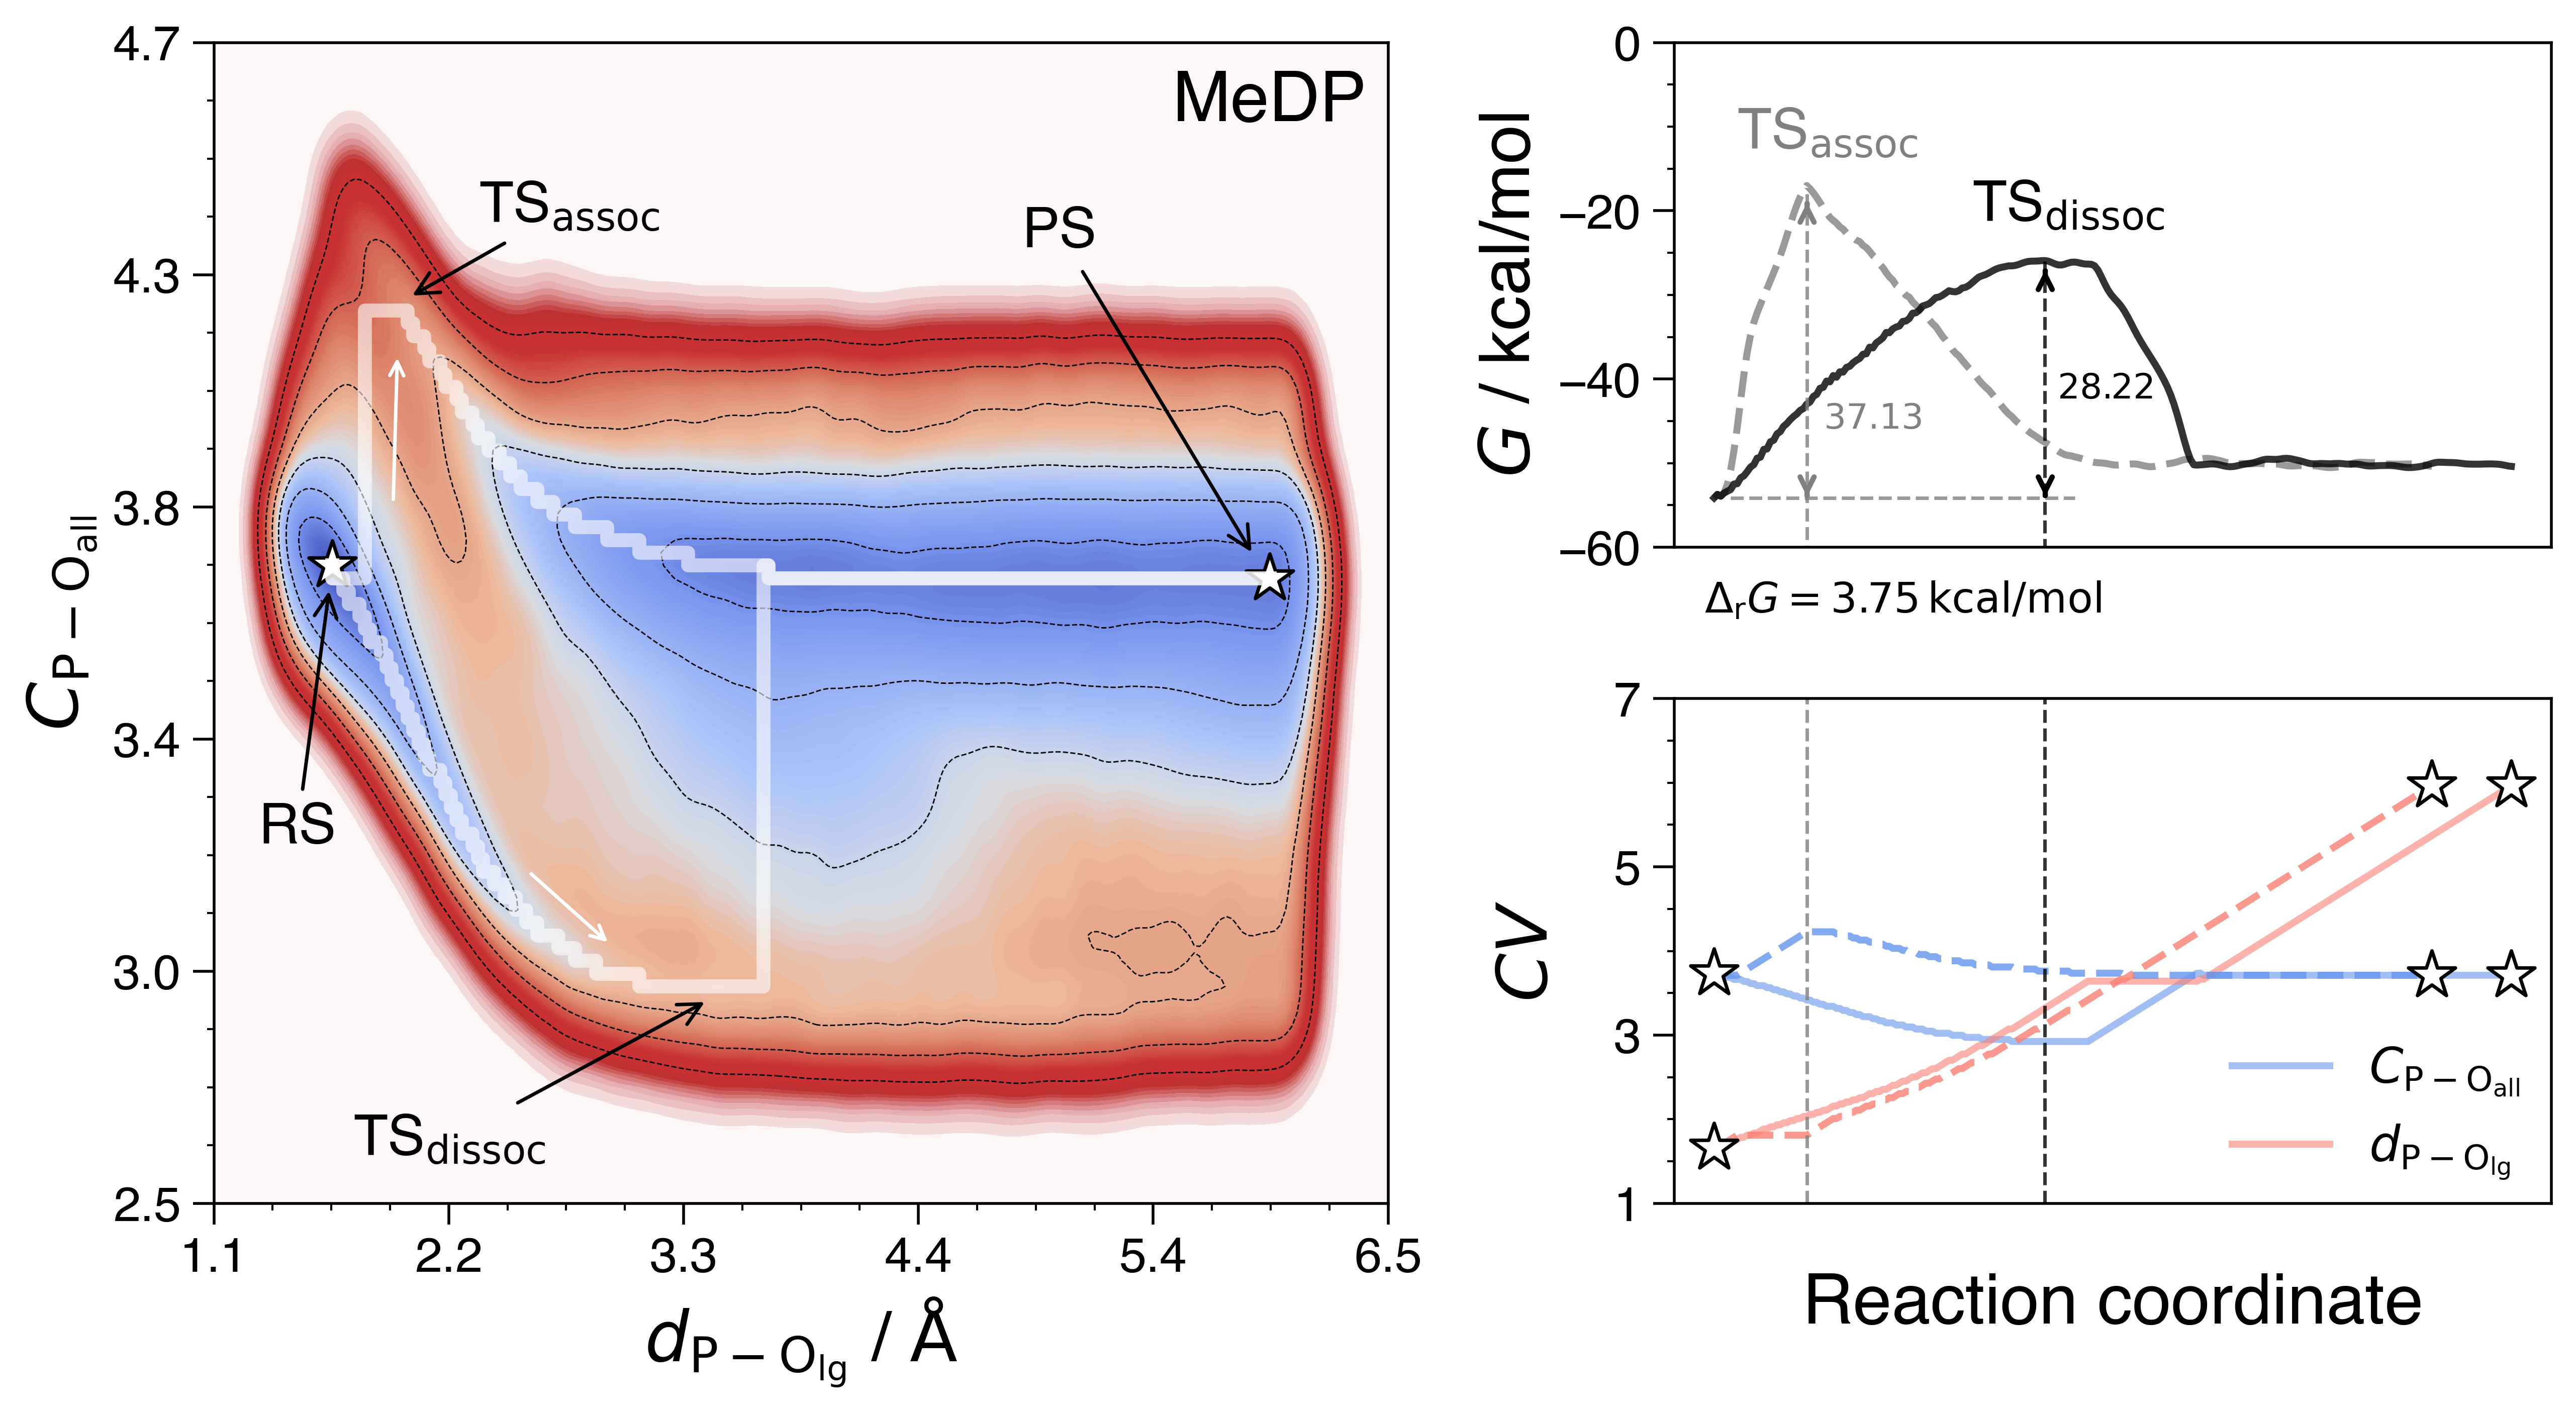
\includegraphics[width=0.9\textwidth]{Figures/4_Results/results_MeDP_300K_fes_mfep.png}
    \caption{FES and MFEP MeDP 300K}
    \label{fig:medp_300k_fes_mfep}
\end{figure}


\subsection{Proton transfer mechanism}



%%%%%%%%%%%%%%%%%%%%%%%%%%%%%%%%%%%%%%%%%%%%%%%%%%%%%%%%%%%%%%%%%%%%%%%%%%%%%%%%
\clearpage
\section{Reaction mechanism for methyl diphosphate dianion}

% MeHDP
% RS -44.839340149
% PS -57.088073014

% TSassoc -14.408871871 31
% CN d
% 4.19 1.89

% TSdissoc -15.936543814 141
% CN d
% 2.89 4.23


\subsection{Minimum free energy path}

\begin{figure}[ht]
    \centering
    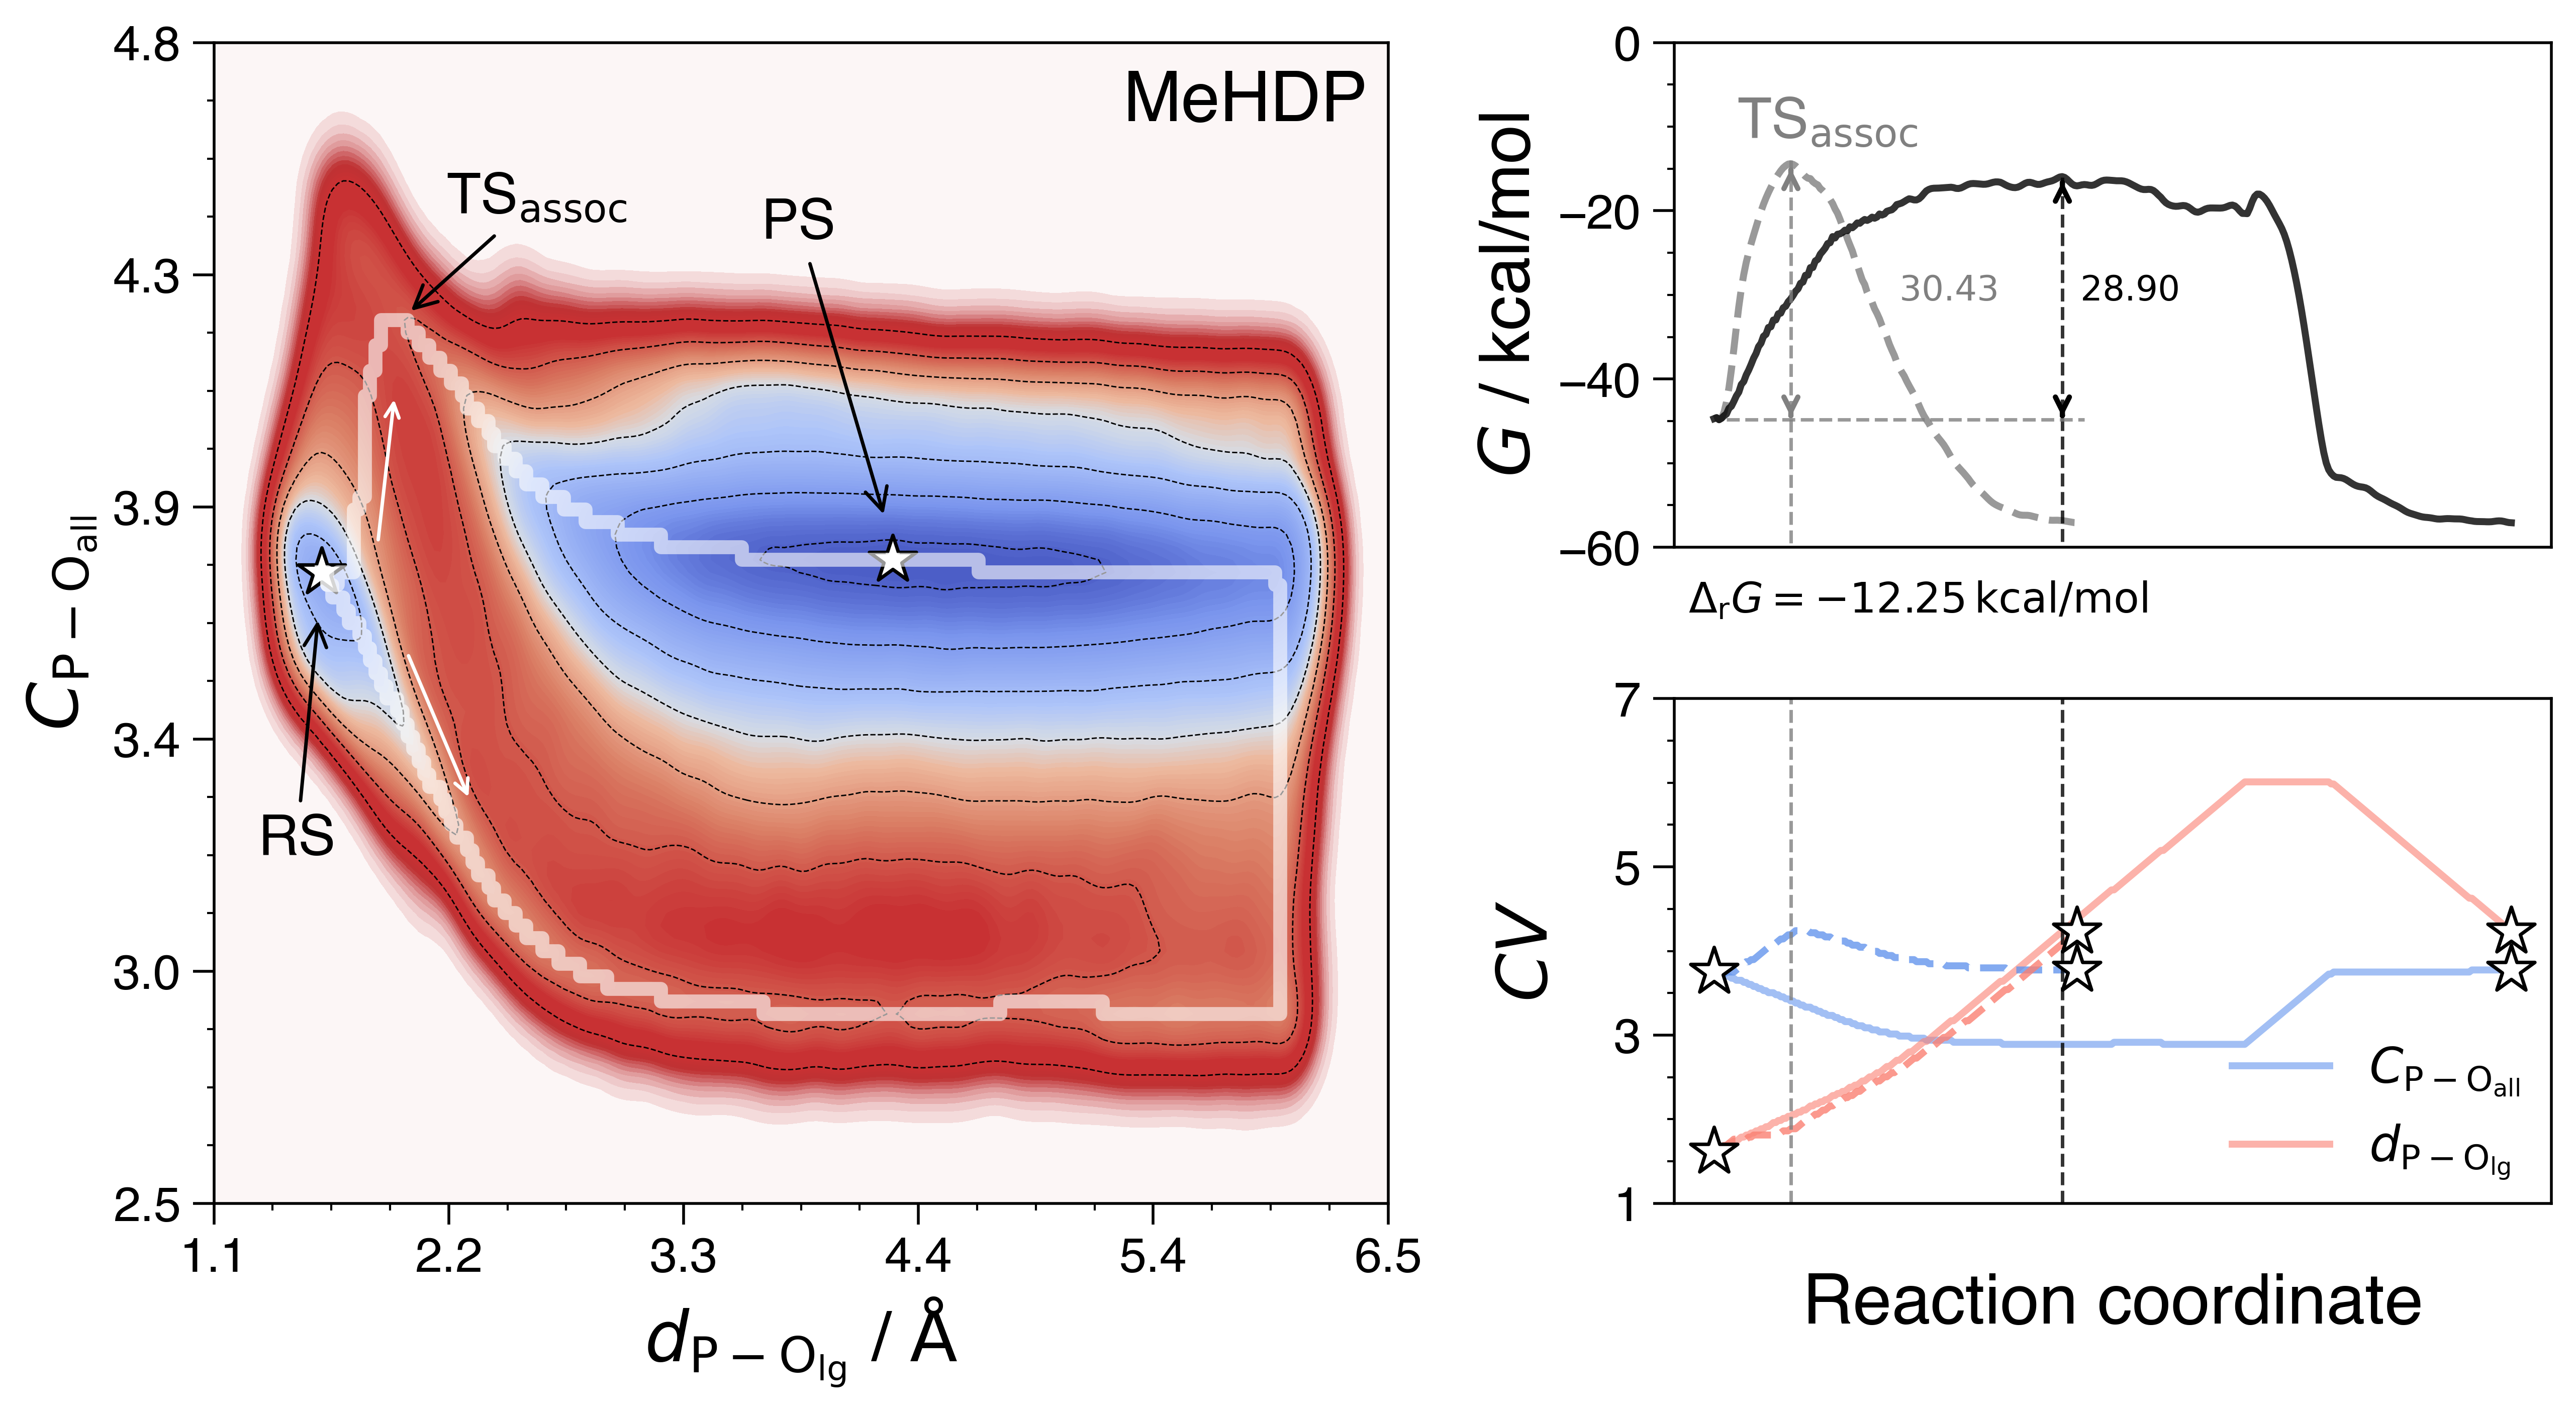
\includegraphics[width=0.9\textwidth]{Figures/4_Results/results_MeHDP_300K_fes_mfep.png}
    \caption{FES and MFEP MeHDP 300K}
    \label{fig:mehdp_300k_fes_mfep}
\end{figure}


\subsection{Proton transfer mechanism}



